\documentclass[11pt,a4paper]{article}

% ---------------------------------------------------------------- layout
\usepackage[a4paper,top=2.2cm,bottom=2.3cm,left=2.2cm,right=2.2cm,headheight=14pt]{geometry}
\usepackage[T1]{fontenc}
\usepackage[utf8]{inputenc}
\usepackage{amsmath}
\usepackage{mathptmx}
\usepackage[scaled=0.92]{helvet}
\usepackage{inconsolata}
\usepackage{microtype}
\usepackage{graphicx}
\usepackage{xcolor}
\usepackage{tikz}
\usetikzlibrary{arrows.meta,positioning,calc}
\usepackage{pgfplots}
\pgfplotsset{compat=1.18}
\usepackage{booktabs}
\usepackage{tabularx}
\usepackage{array}
\usepackage{multirow}
\usepackage{caption}
\usepackage{subcaption}
\usepackage{float}
\usepackage{placeins}
\usepackage{enumitem}
\usepackage{titlesec}
\usepackage{fancyhdr}
\usepackage{lastpage}
\usepackage{needspace}
\usepackage{fancyvrb}
\usepackage{xurl}
\usepackage[hidelinks]{hyperref}


\setlength{\parindent}{0pt}
\setlength{\parskip}{5pt plus 1pt}
\setlist{itemsep=2pt,topsep=3pt,parsep=0pt,leftmargin=*}
\captionsetup{font=small,labelfont=bf,skip=5pt}
\renewcommand{\arraystretch}{1.1}
\newcolumntype{L}{>{\raggedright\arraybackslash}X}
\newcolumntype{C}{>{\centering\arraybackslash}X}
\newcolumntype{P}[1]{>{\raggedright\arraybackslash}p{#1}}
\setcounter{tocdepth}{1}

\titleformat{\section}{\sffamily\Large\bfseries}{\thesection}{0.6em}{}
\titleformat{\subsection}{\sffamily\large\bfseries}{\thesubsection}{0.6em}{}
\titleformat{\subsubsection}{\sffamily\normalsize\bfseries}{\thesubsubsection}{0.6em}{}
\titlespacing*{\section}{0pt}{12pt}{5pt}
\titlespacing*{\subsection}{0pt}{9pt}{3pt}
\titlespacing*{\subsubsection}{0pt}{7pt}{2pt}

\pagestyle{fancy}
\fancyhf{}
\fancyhead[L]{\sffamily\small EC8203 Mini Project: FleetPulse}
\fancyhead[R]{\sffamily\small Lambda architecture for a ride-hailing fleet}
\fancyfoot[C]{\sffamily\small Page \thepage\ of \pageref{LastPage}}
\renewcommand{\headrulewidth}{0.4pt}

\newcommand{\code}[1]{\texttt{#1}}
% alert names are identifiers, never split them at a line end
\hyphenation{ServiceDown SpeedLayerStale NoTelemetryIngested StreamingQueryDown KafkaConsumerLagHigh EndToEndLatencyHigh InvalidEventRateHigh BatchLayerBehind ExpenseFeedMissing VehicleIdleTooLong VehiclesBecomingUnprofitable FleetPulse PostgreSQL}
% generated by report/tools/make_numbers.py - do not edit by hand
\newcommand{\NumDays}{15}
\newcommand{\RunMinutes}{178}
\newcommand{\LatencyAvg}{2.3}
\newcommand{\EventsPerDay}{11,400}
\newcommand{\LateEventsPerDay}{174}
\newcommand{\TripsPerDay}{463}
\newcommand{\BatchSecondsAvg}{20}
\newcommand{\ReportDay}{15 Sep}
\newcommand{\LastDay}{2026-09-15}

% narrative sentences written after reading the results of the run (values from the database and the drill log)
\newcommand{\LiveText}{The picture was taken at 15:02 on simulated Thursday 17 September, while the system was
still running after the 15 measured days. At that moment 27 of the 30 vehicles were online. 37\% of them were
carrying a passenger and 52\% were waiting for a ride. The fleet had finished 245 trips that day and earned
236,296 LKR in fares. No vehicle had an open idle alert, and 8 vehicles had lost money so far that day (live
fares minus fuel and the part of the daily maintenance cost used up so far).}

\newcommand{\BusinessText}{Over the 15 days the fleet made 150,599 LKR net profit per day on average, and the
vehicles carried a passenger in 39.6\% of their online time. The five vehicles with special profiles
(Section~\ref{sec:sources}) behaved as planned, and the pipeline found each of them without being told:
\begin{itemize}
\item \textbf{V007} made 6,199 LKR on day 1 but lost 17,830 LKR on day 15. Its fuel cost rose from 19.0 to
44.0 LKR per km, and its trips fell from 14 to 4 a day. It was first flagged as becoming unprofitable on day 3,
its first day with a loss. From day 4 to day 10 the report listed it as unprofitable only, because each day
had a service bill or a steady loss. From day 11 the loss grew again every day, so the flag came back.
\item \textbf{V013} lost money only on its four service days, when maintenance cost 21,000 to 26,000 LKR. It
was never flagged as becoming unprofitable, because one large bill is not a falling trend.
\item \textbf{V026} made a profit on every day except its one service day, so a profit rule alone would miss
it. But it claimed 184 km a day while the GPS showed only 138 km, and the report listed it every day for this
gap (28 to 40\%).
\item \textbf{V021} and \textbf{V027} made 2,654 LKR a day, less than half of the 6,267 LKR of the 23
vehicles with no special profile or night shift. They were idle for 514 minutes a day (others: 349) and made
9.7 trips (others: 17.0).
\end{itemize}
The pipeline also found one story that we did not plan. \textbf{V030} works at night, when there are few
rides. It made only 588 LKR a day on average and was flagged three times (days 5, 8 and 14). In total the batch
layer raised 9 ``becoming unprofitable'' flags in 15 days, 6 for V007 and 3 for V030, and none for any other
vehicle.}

\newcommand{\ReconText}{On an average day the speed layer missed about two trips, and its fares were 0.42\%
below the exact batch value (never more than 1.11\%). So the live numbers are good enough to act on during the
day, and the batch numbers are the final answer for money.}

\newcommand{\HealthText}{Every DAG run succeeded. Two runs needed the automatic retry of the sensor
\code{wait\_for\_expense\_file}, both times because we recreated a container (Airflow once and PostgreSQL once)
while the sensor was running. The PostgreSQL restart also stopped the Spark streaming job. Docker restarted
it, and its four queries continued from their checkpoints within about 20 seconds.

We used the recompute path for a real reason. We changed the profit rule so that a service day does not count
as a falling trend, and then triggered the DAG for days 1 to 13 through the Airflow REST API with the
\code{sim\_date} parameter. The 13 runs took 7 minutes and 1 second in total, and the ``becoming unprofitable''
flags for those days fell from 20 to 6. A rule change in a Lambda system is only a rerun of the batch layer.

The alerts also caught one real mistake. At the start of the long run we lowered the memory of the Spark
streaming driver, and Spark refused to start because it needs at least 450\,MB. SpeedLayerStale and
ServiceDown (Spark) fired within two minutes of the first error, and both were resolved less than four
minutes after it, once we set the memory back to 512\,MB.}

\newcommand{\DrillText}{Figure~\ref{fig:health} shows the result. Within 12 seconds Prometheus marked
ServiceDown (stream-producer) and NoTelemetryIngested as pending. Both were firing at 73 seconds, because the
rules wait one minute to avoid false alarms. The API webhook received ServiceDown at 81 seconds. It did not
receive NoTelemetryIngested, because the inhibition rule hides it while the producer is known to be down. So
the team gets one clear message instead of two. SpeedLayerStale was firing at 113 seconds and reached the
webhook at 122 seconds. This is correct, because the live dashboards had stopped changing. We started the
producer again at 215 seconds. All alerts cleared within 18 seconds, and the ``resolved'' messages arrived 27
and 47 seconds after the restart. The simulator does not send the events of the time when it was stopped, so
the drill day (16 September) has a gap of about seven simulated hours. For this reason the results in
Section~\ref{sec:daily} stop at 15 September.}


\begin{document}

% ---------------------------------------------------------------- title page
\begin{titlepage}
\centering
\vspace*{0.2cm}

\includegraphics[height=3.4cm]{figures/university_logo.jpg}\par
\vspace{0.5cm}
{\sffamily\large UNIVERSITY OF RUHUNA\par}
\vspace{2pt}
{\sffamily\large Faculty of Engineering\par}
\vspace{1.3cm}
{\sffamily\Large EC8203 Applied Big Data Engineering\par}
\vspace{4pt}
{\sffamily\large Mini Project Report\par}
\vspace{1.8cm}
{\sffamily\fontsize{30}{36}\selectfont\bfseries FleetPulse\par}
\vspace{0.5cm}
{\sffamily\Large A Lambda Architecture for Real-Time Fleet Utilisation\\[2pt] and Daily Vehicle Profitability\par}
\vspace{0.6cm}
{\sffamily\large Use Case 1: Ride-Hailing Fleet Operations\par}
\vfill
{\sffamily\large Group members\par}
\vspace{8pt}
\begin{tabular}{ll}
\toprule
\textbf{Name} & \textbf{Registration number} \\
\midrule
Arivanan V. & EG/2021/4414 \\
Shageethpratheep V. & EG/2021/4809 \\
Shayanthavi T. & EG/2021/4811 \\
\bottomrule
\end{tabular}
\vfill
{\sffamily\large 30 September 2026\par}
\vspace*{0.4cm}
\end{titlepage}

% ---------------------------------------------------------------- abstract
\section*{Abstract}
This report describes FleetPulse, a small but complete data platform for a ride-hailing company in
Colombo. The platform answers two business questions. How busy is the fleet, and how much does it earn
in each area right now? Which vehicles are becoming unprofitable once yesterday's fuel and maintenance
costs are added? We chose a Lambda architecture. The speed layer uses Apache Kafka and Spark Structured
Streaming and shows live numbers a few seconds after an event happens. The batch layer is started by
Apache Airflow once per simulated day. It recomputes the whole day from raw data with Spark and joins it
with the cost file from our fuel and garage partners. All results are stored in PostgreSQL and served by a
FastAPI service, three Grafana dashboards and a daily HTML report. Structured logs, Prometheus metrics and
14 alert rules make every stage observable. The whole system starts with one Docker Compose command on a
laptop. In our test run of \NumDays{} simulated days, the speed layer kept the end-to-end latency near
\LatencyAvg{} seconds, and the batch layer found every loss-making vehicle and explained why, including one
vehicle whose profit fell day after day.


\section{Introduction}

\subsection{Use case}
We chose Use Case 1, Ride-Hailing Fleet Operations. Our operator, FleetPulse, runs 30 vehicles in
Colombo: 13 tuk-tuks, 10 mini cars and 7 cars. The operator owns the vehicles. It pays for fuel and
maintenance and gives each driver 30\% of the fares. We divided the city into 12 zones, such as
Fort-Pettah, Kollupitiya, Borella, Wellawatte and Nugegoda. The use case asks one question with two parts:

\begin{quote}\itshape
``What is fleet utilization and earnings by area/time-of-day right now, and which vehicles are becoming
unprofitable once yesterday's fuel/maintenance costs are factored in?''
\end{quote}

The first part needs fresh numbers within seconds. The second part needs exact money numbers, but only once
a day. This difference is the main reason for our design.

\subsection{Business requirements}
Table~\ref{tab:requirements} lists the requirements we took from the use case. The last two columns show how
fast and how exact each answer must be.

\begin{table}[!htb]
\centering\small
\caption{Business requirements taken from the use case.}
\label{tab:requirements}
\begin{tabularx}{\textwidth}{@{}l L P{2.9cm} P{3.6cm}@{}}
\toprule
\textbf{ID} & \textbf{Requirement} & \textbf{How fast} & \textbf{How exact} \\
\midrule
R1 & Live fleet status: vehicles online, on a trip and idle & a few seconds & approximate is fine \\
R2 & Utilisation and fares by zone and hour of day & seconds & small errors are fine \\
R3 & Alert when a vehicle stays idle for a long time & simulated minutes & one alert per idle period \\
R4 & Daily profit of each vehicle after fuel and maintenance & once per day & exact, it is money \\
R5 & Find vehicles that are becoming unprofitable & once per day & exact, needs history \\
R6 & Recompute a day when late data or a corrected file arrives & on request & exact and repeatable \\
R7 & Show the health of every pipeline stage & seconds & logs, metrics and alerts \\
R8 & Run on one laptop with 8\,GB of memory & always & low memory and CPU \\
\bottomrule
\end{tabularx}
\end{table}

\subsection{Simulated clock and assumptions}
A real business day is long. To show many days in a short demo, we compress time. One real second is two
simulated minutes (a speed-up of 120), so 30 real seconds are one simulated hour and 12 real minutes are one
simulated day. The simulation starts on Tuesday 1~September~2026 at 06:00, so day~1 is 18 hours long and
later days are 24 hours long. All simulated times are Sri Lanka local time. The clock is stored in one
database row, so every container agrees on the simulated ``now''. If the whole system stops for more than
five minutes, simulated time pauses and continues after the restart.

We also made these assumptions:
\begin{itemize}
\item Both data sources are Python scripts. The numbers are realistic but they are not real company data.
\item Money is in Sri Lankan rupees (LKR). Petrol costs about LKR 305 per litre.
\item The daily cost file arrives 20 to 90 simulated minutes after midnight (10 to 45 real seconds).
\item Kafka, Spark and PostgreSQL each run as a single node. This is enough for about 30 events per second.
\end{itemize}

\section{Architecture decision: Lambda or Kappa}

\subsection{The two options}
Both architectures keep raw events in an append-only store and build views from them \cite{kleppmann2017}. They differ in how
they compute and recompute those views.

\textbf{Lambda} has three layers \cite{marz2015}. The \emph{batch layer} keeps all raw data in a master
dataset that never changes and recomputes views from it on a schedule. The \emph{speed layer} processes
new events as they arrive and covers the time until the next batch run. The \emph{serving layer} merges
both kinds of views for users.

\textbf{Kappa} has only a stream layer \cite{kreps2014}. All data, old and new, is a stream in a log such
as Kafka. There is one processing job. To recompute, a second copy of the job reads the log again from an
old offset, and users switch to it when it catches up.

\subsection{Comparing the options with our requirements}
Table~\ref{tab:lambda-kappa} compares the two options against the requirements in
Table~\ref{tab:requirements}.

\begin{table}[!htb]
\centering\small
\caption{Lambda and Kappa compared for our use case. The last column shows which option fits us better.}
\label{tab:lambda-kappa}
\begin{tabularx}{\textwidth}{@{}P{2.6cm} L L P{1.2cm}@{}}
\toprule
\textbf{Criterion} & \textbf{Lambda} & \textbf{Kappa} & \textbf{Better} \\
\midrule
Latency (R1 to R3) & The speed layer updates every 5 to 10 seconds. & The stream job updates every few seconds. & equal \\
Exact money (R4, R5) & The batch layer reads the complete day after late events and the cost file have arrived. & Windows close at a watermark. Later events are dropped or need extra update logic after results are published. & Lambda \\
Daily cost file & Read directly as a batch input. & Must become a stream and wait in state until a full day of trips is ready. & Lambda \\
Recompute a day (R6) & Rerun the Airflow DAG for that day from Parquet files. & Replay the Kafka log from an old offset with a second copy of the job. & Lambda \\
Storage cost & Cheap compressed Parquet files keep all history. & Kafka must keep weeks or months of events. & Lambda \\
Code & Two paths (stream and batch) that can drift apart. & One code path. & Kappa \\
Operations & More parts: Airflow, a batch job and merge views. & Fewer parts. & Kappa \\
Consistency & Live views are temporary. Batch views become the truth for finished days. & One view, but its accuracy depends on the watermark. & Lambda \\
\bottomrule
\end{tabularx}
\end{table}

\subsection{Our decision: Lambda}
We chose the Lambda architecture for five reasons.
\begin{enumerate}
\item \textbf{Two very different sources.} One source is a continuous stream and the other is one file
per day. The daily file is a natural batch input, and the daily report is a natural batch output.
\item \textbf{Money must be exact.} Vehicles in our simulation sometimes lose signal for 20 to 60 simulated
minutes and then send all the old events at once. In our run, about \LateEventsPerDay{} events per day
arrived more than 10 simulated minutes late. To keep its state small, the speed layer closes each window
soon after it ends, so events that arrive later are lost. The batch layer starts only after the day and a
grace period have ended, so it counts every event, removes repeats over the whole day and joins the complete
cost file.
\item \textbf{Recomputing is cheap and simple.} One simulated day has about \EventsPerDay{} events, which is
only a few megabytes of Parquet. If a partner sends a corrected cost file, we rerun the DAG for that day.
Nothing in Kafka has to be replayed and Kafka can keep a short retention.
\item \textbf{Latency is still low.} The speed layer writes to PostgreSQL every 5 to 10 seconds, so the
live dashboard meets requirements R1 to R3.
\item \textbf{The tools fit.} Airflow is built for scheduled batch jobs, and Spark can run both the
streaming job and the batch job with the same API.
\end{enumerate}

\subsection{The rejected alternative: Kappa}
In a Kappa design, the batch simulator would send its cost rows into a Kafka topic. One Spark streaming job
would keep a full day of trip totals per vehicle in its state and join them with the cost rows when they
arrive. To fix a day, we would replay the log from an old offset. We rejected this design because the join
needs a whole day of state for every vehicle, because late events after the watermark would change money
numbers that were already published, and because replay needs Kafka to keep all history. Kappa does have a
real advantage: one code path and fewer moving parts. If costs arrived as live events, or if the business
only needed live numbers, Kappa would be the better choice.

\subsection{How we reduce the weak points of Lambda}
The main problem of Lambda is keeping two code paths correct and in step. We reduce it in four ways.
\begin{itemize}
\item \textbf{One engine.} Both layers use Spark 4.1 and the same DataFrame API.
\item \textbf{Shared code.} Parsing, validation, the zone lookup, the metric definitions and the profit rules
live in one module (\code{fleet\_transforms.py}) that both layers import. A unit test checks that the Spark
version and the Python version of the profit rules give the same answer.
\item \textbf{A clear hand-over.} For a finished day the serving views show batch results only. The DAG then
deletes speed-layer rows for older days (Figure~\ref{fig:handover}).
\item \textbf{Reconciliation.} After each batch run we compare the speed and batch totals of the day and store
the difference (Section~\ref{sec:reconciliation}).
\end{itemize}

\begin{figure}[!htb]
\centering
% Timeline of the Lambda hand-over from the speed layer to the batch layer
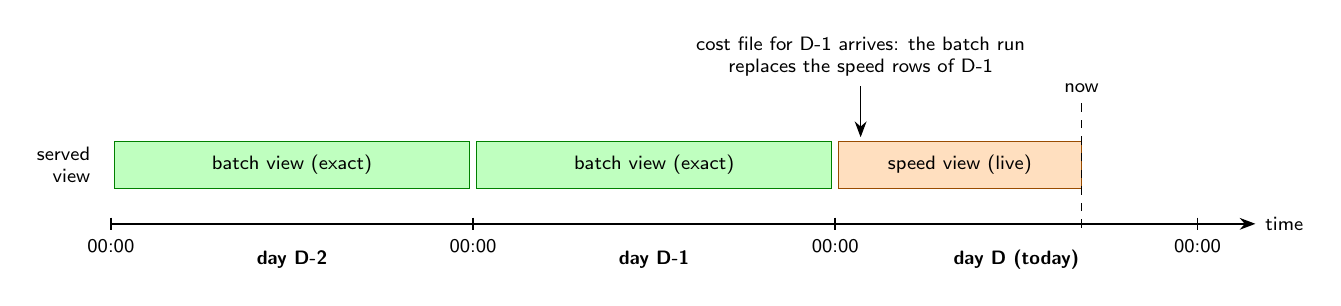
\begin{tikzpicture}[font=\sffamily\scriptsize, x=0.92cm, y=1cm]
% axis
\draw[-{Stealth[length=2mm]}, line width=0.6pt] (0,0) -- (15.8,0) node[right] {time};
\foreach \x in {0, 5, 10, 15} { \draw[line width=0.6pt] (\x,0.08) -- (\x,-0.08); }
\node[below] at (0,-0.08) {00:00};
\node[below] at (5,-0.08) {00:00};
\node[below] at (10,-0.08) {00:00};
\node[below] at (15,-0.08) {00:00};
\node[font=\sffamily\scriptsize\bfseries] at (2.5,-0.45) {day D-2};
\node[font=\sffamily\scriptsize\bfseries] at (7.5,-0.45) {day D-1};
\node[font=\sffamily\scriptsize\bfseries] at (12.5,-0.45) {day D (today)};
% served views
\node[anchor=east, align=right] at (-0.15,0.75) {served\\view};
\fill[green!25, draw=green!50!black, line width=0.4pt] (0.05,0.45) rectangle (4.95,1.05);
\node at (2.5,0.75) {batch view (exact)};
\fill[green!25, draw=green!50!black, line width=0.4pt] (5.05,0.45) rectangle (9.95,1.05);
\node at (7.5,0.75) {batch view (exact)};
\fill[orange!25, draw=orange!60!black, line width=0.4pt] (10.05,0.45) rectangle (13.4,1.05);
\node at (11.72,0.75) {speed view (live)};
% now marker
\draw[dashed, line width=0.6pt] (13.4,-0.05) -- (13.4,1.55);
\node[above] at (13.4,1.55) {now};
% batch run for D-1
\draw[-{Stealth[length=2mm]}, line width=0.6pt] (10.35,1.75) -- (10.35,1.10);
\node[above, align=center] at (10.35,1.75) {cost file for D-1 arrives: the batch run\\replaces the speed rows of D-1};
\end{tikzpicture}

\caption{How the serving layer uses the two layers over time. Finished days come from the batch layer.
Today comes from the speed layer until the batch run for today replaces it after midnight.}
\label{fig:handover}
\end{figure}

\section{System design}

\subsection{Architecture overview}
Figure~\ref{fig:architecture} shows the whole system, from the two sources to the three ways of serving
results. Every box runs in its own Docker container, and one Docker Compose file starts all of them.

\begin{figure}[!htb]
\centering
% FleetPulse architecture (Lambda). Drawn at text width (16 cm), no scaling needed.
\begin{tikzpicture}[
  font=\sffamily\scriptsize,
  box/.style={draw=black!55, rounded corners=2pt, align=center, inner sep=2.5pt, line width=0.5pt},
  arrow/.style={-{Stealth[length=2mm]}, line width=0.7pt, draw=black!70},
  dashedarrow/.style={arrow, dashed},
  lbl/.style={font=\sffamily\tiny, text=black, inner sep=2.4pt},
  layer/.style={font=\sffamily\scriptsize\bfseries, text=black},
]
% ---- layer titles
\node[layer] at (1.25, 8.00) {SOURCES};
\node[layer] at (4.60, 8.00) {INGESTION};
\node[layer] at (8.30, 8.00) {PROCESSING};
\node[layer] at (11.90, 8.00) {STORAGE};
\node[layer] at (14.90, 8.00) {SERVING};

% ---- sources (x 0.10 to 2.30)
\node[box, fill=black!6, text width=2.2cm, minimum height=1.4cm] (ss) at (1.25, 6.40)
  {\textbf{Stream simulator}\\Python, 30 vehicles,\\one ping per second};
\node[box, fill=black!6, text width=2.2cm, minimum height=1.4cm] (bs) at (1.25, 2.50)
  {\textbf{Batch simulator}\\Python, cost file\\once per day};

% ---- ingestion (x 3.20 to 5.90)
\node[box, fill=orange!14, text width=2.75cm, minimum height=2.3cm] (kafka) at (4.60, 6.40)
  {\textbf{Apache Kafka 4.3}\\KRaft, one broker\\[2pt]topic\\\texttt{fleet.telemetry.raw}\\6 partitions,\\key = vehicle id\\[2pt]+ dead-letter topic};
\node[box, fill=orange!14, text width=2.75cm, minimum height=1.4cm] (land) at (4.60, 2.50)
  {\textbf{Landing zone}\\daily CSV file and\\manifest (SHA-256)};

% ---- processing (x 6.75 to 9.85)
\node[box, fill=teal!14, text width=2.9cm, minimum height=2.3cm] (speed) at (8.30, 6.40)
  {\textbf{Speed layer}\\Spark 4.1 Structured\\Streaming: validate,\\de-duplicate, watermark,\\zone join, 1 h and 1 day\\windows, idle alerts};
\node[box, fill=violet!12, text width=2.9cm, minimum height=0.9cm] (lake) at (8.30, 4.45)
  {\textbf{Master dataset}\\immutable raw Parquet};
\node[box, fill=blue!10, text width=2.9cm, minimum height=1.9cm] (batch) at (8.30, 2.50)
  {\textbf{Batch layer}\\Airflow 3.3 DAG runs a\\Spark 4.1 batch job\\once per day: exact\\recompute and join\\with partner costs};

% ---- storage (x 10.75 to 13.05)
\node[box, fill=violet!12, text width=2.1cm, minimum height=5.4cm] (pg) at (11.90, 4.45)
  {\textbf{PostgreSQL 17}\\[5pt]\texttt{speed.*}\\real-time views\\[5pt]\texttt{batch.*}\\exact daily views\\[5pt]\texttt{serving.*}\\merge views\\[5pt]\texttt{ops.*}\\audit, alerts, clock};

% ---- serving (x 13.80 to 16.00)
\node[box, fill=green!12, text width=2.0cm, minimum height=1.0cm] (api) at (14.90, 6.40)
  {\textbf{FastAPI}\\REST and /metrics};
\node[box, fill=green!12, text width=2.0cm, minimum height=1.0cm] (graf) at (14.90, 4.45)
  {\textbf{Grafana 12}\\3 dashboards};
\node[box, fill=green!12, text width=2.0cm, minimum height=1.0cm] (rep) at (14.90, 2.50)
  {\textbf{Daily report}\\HTML and CSV};

% ---- data flow
\draw[arrow] (ss) -- node[lbl, above] {JSON} (kafka);
\draw[arrow] (kafka) -- node[lbl, above] {stream} (speed);
\draw[arrow] (bs) -- node[lbl, above] {CSV} (land);
\draw[arrow] (land) -- node[lbl, above] {sensor} (batch);
\draw[dashedarrow] (speed) -- node[lbl, right] {raw archive} (lake);
\draw[arrow] (lake) -- node[lbl, right] {one day} (batch);
\draw[arrow] (speed.east) -- node[lbl, above] {upsert} (speed.east -| pg.west);
\draw[arrow] (batch.east) -- node[lbl, above] {one txn} (batch.east -| pg.west);
\draw[arrow] (pg.east |- api.west) -- (api.west);
\draw[arrow] (pg.east |- graf.west) -- (graf.west);
\draw[arrow] (pg.east |- rep.west) -- (rep.west);

% ---- observability band (x 0.10 to 16.00)
\node[box, fill=yellow!16, text width=15.6cm, minimum height=0.8cm, anchor=west] (obs) at (0.10, 0.60)
  {\textbf{Observability:} JSON logs from every stage \,\textbullet\, Prometheus 3 metrics (producers, Spark listener,
   API, Airflow via StatsD) \,\textbullet\, 14 alert rules $\rightarrow$ Alertmanager $\rightarrow$ API webhook
   \,\textbullet\, lineage and audit tables};
\foreach \n in {bs, land, batch, pg, rep} {
  \draw[densely dotted, draw=black!45, line width=0.6pt] (\n.south) -- (\n.south |- obs.north);
}
\end{tikzpicture}

\caption{FleetPulse architecture. The top row is the streaming path and the bottom row is the daily batch
path. Both meet in PostgreSQL. The dotted lines show that every stage sends logs and metrics.}
\label{fig:architecture}
\end{figure}

\textbf{Streaming path.} The stream simulator sends a JSON event to Kafka for every vehicle every real
second. Spark Structured Streaming reads the topic with four queries. Three of them clean the events and
update the real-time tables in PostgreSQL. The fourth writes every raw record, unchanged, to the master
dataset in Parquet.

\textbf{Batch path.} Once per simulated day the batch simulator drops a CSV file and a manifest into the
landing zone. An Airflow sensor finds the file, checks it and copies it into the master dataset. Airflow
then starts a Spark batch job. The job reads one full day of raw events, removes bad and repeated records,
joins the day with the cost file and writes exact results to PostgreSQL in a single transaction.

\textbf{Serving.} PostgreSQL views merge the two layers. The FastAPI service, the Grafana dashboards and the
daily report all read from these tables and views.

\subsection{Data sources}
The streaming source sends one JSON event per Kafka message with the fields \code{event\_id} (a UUID, also
sent as the Kafka header \code{trace\_id}), \code{event\_type} (\code{ping} every 2 simulated minutes,
\code{trip\_start} or \code{trip\_end}), \code{event\_ts} (simulated time), \code{vehicle\_id},
\code{driver\_id}, \code{trip\_id} (empty when idle), \code{status} (\code{idle}, \code{enroute} to a
pickup or \code{on\_trip}), \code{lat}, \code{lon}, \code{speed} (km/h), \code{odometer\_km} and
\code{fare} (the running fare, or the final fare on \code{trip\_end}). A \code{trip\_end} event also carries
the pickup point, trip distance and duration. We added \code{event\_id}, \code{event\_type} and
\code{odometer\_km} to the fields listed in the brief.

The daily source is a CSV file from the fuel and garage partners, with a manifest. It has one row per
vehicle and day with the fields \code{record\_id}, \code{expense\_date}, \code{vehicle\_id},
\code{partner\_id}, \code{fuel\_litres}, \code{fuel\_cost}, \code{maintenance\_cost} (upkeep, wear and any
service bill), \code{distance\_covered} (kilometres reported by the partner, which we check against GPS) and
\code{service\_flag} (\code{Y} on a day with a garage service).

To test the cleaning logic, both sources add problems on purpose: about 1\% of events are sent twice,
0.5\% of pings are broken (bad JSON, missing ids, a GPS point at 0,0, negative speed and more), and
vehicles sometimes lose signal and send their events late. Most daily files also contain a repeated row, a
row for an unknown vehicle, a bad number or a missing vehicle id.

\subsection{Kafka design}
We use two topics. \code{fleet.telemetry.raw} has six partitions and carries all telemetry, which the speed
layer reads and archives for the batch layer. \code{fleet.telemetry.dlq} has one partition. It is the
dead-letter queue, which keeps invalid events with the reason for checks and replay. Messages are keyed by
\code{vehicle\_id}, so all events of one vehicle go to the same partition and stay in order. This order
matters for idle streaks and trips. Six partitions allow up to six consumers to read in parallel. The
producer uses \code{acks=all} with the idempotent producer switched on, so retries after a network error never
create duplicates in Kafka. It also uses lz4 compression and a 20~ms linger time to send small batches.

\subsection{Storage design}
The \textbf{master dataset} is a folder of Parquet files that we never change, only add to. Raw telemetry is
partitioned by the simulated date (\code{lake/raw/telemetry/event\_date=2026-09-01/}) and written by the
Spark file sink, whose metadata log makes each write exactly-once. The partner files are kept in
\code{lake/raw/expenses/}. The batch layer also keeps its own results in \code{lake/curated/} and reads the
last two days from there to find profit trends.

\textbf{PostgreSQL 17} is the serving store. We chose it because the views are small (a few hundred rows per
day), and it gives SQL, joins, upserts and transactions. It has five schemas: \code{ref} (vehicles and zones),
\code{speed} (live zone and vehicle metrics, vehicle state and idle alerts), \code{batch} (exact metrics,
trips, profitability, cost rates, quarantined cost rows and the daily summary), \code{serving} (views that
merge the two layers and the live profit projection) and \code{ops} (simulated clock, micro-batch ledger,
dead letters, run audit trail, alert notifications and reconciliation).

\section{Technology stack and justification}
Table~\ref{tab:stack} lists every major tool, why it fits this use case and what we compared it with. We
chose each tool for a need of the fleet problem, not because it is popular. All versions are the current
stable releases in September 2026 \cite{spark,kafka,airflow}.

\begin{table}[!htb]
\centering\small
\caption{Technology stack.}
\label{tab:stack}
\begin{tabularx}{\textwidth}{@{}P{1.9cm} P{2.5cm} L P{2.8cm}@{}}
\toprule
\textbf{Layer} & \textbf{Choice} & \textbf{Why it fits our use case} & \textbf{Compared with} \\
\midrule
Ingestion & Apache Kafka 4.3 (KRaft, native image) &
A durable, ordered log. Keys keep each vehicle's events in order, and consumers can re-read by offset after
a failure, so either side can restart without losing data. KRaft needs no ZooKeeper. &
RabbitMQ (no replay by offset), Redpanda \\
Stream processing & Apache Spark 4.1 Structured Streaming &
Event-time windows and watermarks for late GPS data, de-duplication, stream-static joins and checkpoints
for exactly-once processing. The same API runs the batch layer. &
Apache Storm (no batch API, harder state handling) \\
Batch processing & Apache Spark 4.1 (batch) &
Recomputes a day from Parquet with window functions (time in each status, idle streaks) and joins the cost
file, with the module shared with the speed layer. &
Plain SQL in PostgreSQL (raw events would fill the serving store) \\
Orchestration & Apache Airflow 3.3 &
Sensors wait for the file, tasks retry, failures raise an alert, and any day can be rerun with one
parameter. The web UI shows every run. &
cron (no dependencies, retries or run history) \\
Master dataset & Parquet files on a Docker volume &
Columnar, compressed and partitioned by day, so it is cheap to keep forever. In production the same layout
would sit on S3 or HDFS. &
Keeping all history in Kafka \\
Serving store & PostgreSQL 17 &
Results are small (hundreds of rows a day). We need joins for the merge views, upserts for streaming updates
and transactions to publish a whole day at once. &
Cassandra (no joins or multi-row transactions) \\
Serving & FastAPI, Grafana 12, HTML report &
A documented REST API with \code{/metrics}, live dashboards on PostgreSQL and Prometheus, and a report that
is easy to email to managers. &
Streamlit \\
Observability & Prometheus 3, Alertmanager, StatsD exporter, JSON logs &
Metrics from every stage and alert rules. Alertmanager groups and routes alerts, and StatsD brings in the
Airflow metrics. &
Loki and Jaeger (too much memory for our laptop) \\
Deployment & Docker Compose &
One command starts 13 services (11 long-running and 2 set-up jobs) with health checks and memory limits. &
Kubernetes (too heavy for one laptop) \\
\bottomrule
\end{tabularx}
\end{table}

\textbf{Designing for an 8 GB laptop.} Our computer has 8\,GB of memory and Docker gets only about
3.8\,GB. This constraint shaped some choices. We run the three Airflow components in one container with the
LocalExecutor instead of the official set-up with Celery and Redis. Kafka uses the official GraalVM
\emph{native} image, which needed less than 150\,MB in our run instead of about 350\,MB for the Java image. Both Spark jobs
run in local mode with a 512\,MB heap and use only the fast C1 compiler of the Java virtual machine. Without
these changes, the system swapped memory and one batch run took eight minutes.

\section{Implementation}

\subsection{Simulated data sources}
\label{sec:sources}
\textbf{Streaming source.} The file \code{fleet\_model.py} is a small agent-based model. Each vehicle is a
state machine: \emph{offline} $\rightarrow$ \emph{idle} $\rightarrow$ \emph{enroute} to a pickup
$\rightarrow$ \emph{on\_trip} $\rightarrow$ \emph{idle}. Drivers work fixed shifts, and two drivers work at
night so that data never stops. Ride requests arrive at random, and the rate depends on the zone type (city
centre, commercial, residential) and on the hour of the day, with morning and evening peaks. Road speed is
slower in Colombo rush hours. Fares follow simple LKR rules for tuk-tuks, mini cars and cars, with a surge
at peak hours for cars. Every real second each online vehicle sends one ping, and trip start and trip end
events are sent at the moment they happen.

\textbf{Daily-batch source.} At every simulated midnight the model writes a ground-truth file with the true
kilometres of each vehicle. After a random partner delay, \code{batch\_producer.py} turns it into the cost
file: fuel = kilometres divided by fuel efficiency, times the fuel price of the day, and maintenance = daily
upkeep, plus wear per kilometre, plus a service bill on some days. The file is written to a temporary name
and then renamed, so a reader never sees half a file. A manifest with the row count and a SHA-256 checksum is
written last.

Five vehicles have special profiles. These are the stories the pipeline must find without being told:
\begin{itemize}
\item \textbf{V007} (\emph{degrading}): fuel use rises by 15\% and garage time by 2.5 hours every day.
\item \textbf{V013} (\emph{high maintenance}): double upkeep and a service bill on about one day in three.
\item \textbf{V026} (\emph{fuel anomaly}): the partner reports 30 to 40\% more kilometres and fuel than the GPS shows.
\item \textbf{V021} and \textbf{V027} (\emph{idle prone}): the drivers take long breaks and wait a lot.
\end{itemize}

\subsection{Speed layer}
The speed layer is one Spark application (\code{speed\_layer.py}) with the four streaming queries in
Table~\ref{tab:queries}. Each query has its own checkpoint, so after a crash it continues from the exact
Kafka offsets where it stopped.

\begin{table}[!htb]
\centering\small
\caption{Streaming queries of the speed layer.}
\label{tab:queries}
\begin{tabularx}{\textwidth}{@{}P{2.4cm} L P{3.5cm} P{1.1cm}@{}}
\toprule
\textbf{Query} & \textbf{Main operations} & \textbf{Output} & \textbf{Trigger} \\
\midrule
\code{raw\_archive} & copy every record with its Kafka partition, offset and time & Parquet master dataset & 30 s \\
\code{zone\_hourly} & parse, validate, 10-minute watermark, de-duplicate by \code{event\_id}, zone lookup, 1-hour tumbling windows by zone & \code{speed.zone\_hourly} & 10 s \\
\code{vehicle\_daily} & same cleaning, 1-day windows by vehicle (fares and kilometres so far) & \code{speed.vehicle\_daily} & 10 s \\
\code{vehicle\_state} & latest position and status of each vehicle, idle streaks, idle alerts, invalid events & \code{speed.vehicle\_state}, alerts, dead-letter topic & 5 s \\
\bottomrule
\end{tabularx}
\end{table}

\textbf{Cleaning.} Nine validation rules check each event, for example a missing id, a GPS point outside
Sri Lanka, a negative speed or a trip end without a fare. Invalid events go to the dead-letter topic and to
the \code{ops.dead\_letters} table with the list of broken rules. Repeated events are removed with
\code{dropDuplicates\allowbreak Within\allowbreak Watermark} on \code{event\_id}.

\textbf{Enrichment.} GPS points become zone names through a stream-static broadcast join with a small
lookup grid of 0.005-degree cells. Fares count in the zone where the trip started.

\textbf{Late data.} The watermark trails the newest event time by 10 simulated minutes (5 real seconds).
A window stays open until the watermark passes its end, so a late event is still counted if its hour is
open. An event that arrives after its window has closed is dropped, and Spark reports how many. This keeps
the state small. The batch layer later counts these events correctly.

\textbf{Exactly-once writes.} Spark's \code{foreachBatch} can run a micro-batch again after a failure. Each
batch therefore starts its PostgreSQL transaction by inserting its (query name, batch id) pair into
\code{ops.speed\_batches}. If the pair already exists, the batch was committed before and is skipped. The
ledger row and the data rows are committed together, so each micro-batch is applied exactly once.

\textbf{Idle alerts.} For every vehicle we keep \code{idle\_since}, the start of its idle streak. One alert
opens after 90 idle simulated minutes and closes when the vehicle takes a ride or goes offline.

\subsection{Batch layer and orchestration}
\label{sec:batch}
The Airflow DAG \code{fleet\_daily\_batch} (Figure~\ref{fig:dag}) runs once per simulated day. Its steps are:
\begin{enumerate}[itemsep=1pt]
\item \textbf{resolve\_target\_day} picks the oldest day without batch results, or the day given as a
parameter for a rerun.
\item \textbf{wait\_for\_expense\_file} is a sensor. After 1.5 simulated days without a file it fails and
raises an alert.
\item \textbf{validate\_expense\_file} checks the SHA-256 checksum, header and row count against the
manifest, and copies the file into the master dataset.
\item \textbf{wait\_for\_raw\_telemetry} waits until two simulated hours after midnight, so late events of
the day are archived.
\item \textbf{spark\_batch\_recompute} runs \code{spark-submit batch\_layer.py} for the day.
\item \textbf{data\_quality\_checks} tests the published numbers, for example that less than 5\% of events
were invalid.
\item \textbf{build\_daily\_report} writes the HTML and CSV report, and \textbf{purge\_speed\_layer} deletes
speed-layer rows for days that the batch layer now owns.
\end{enumerate}

\begin{figure}[!htb]
\centering
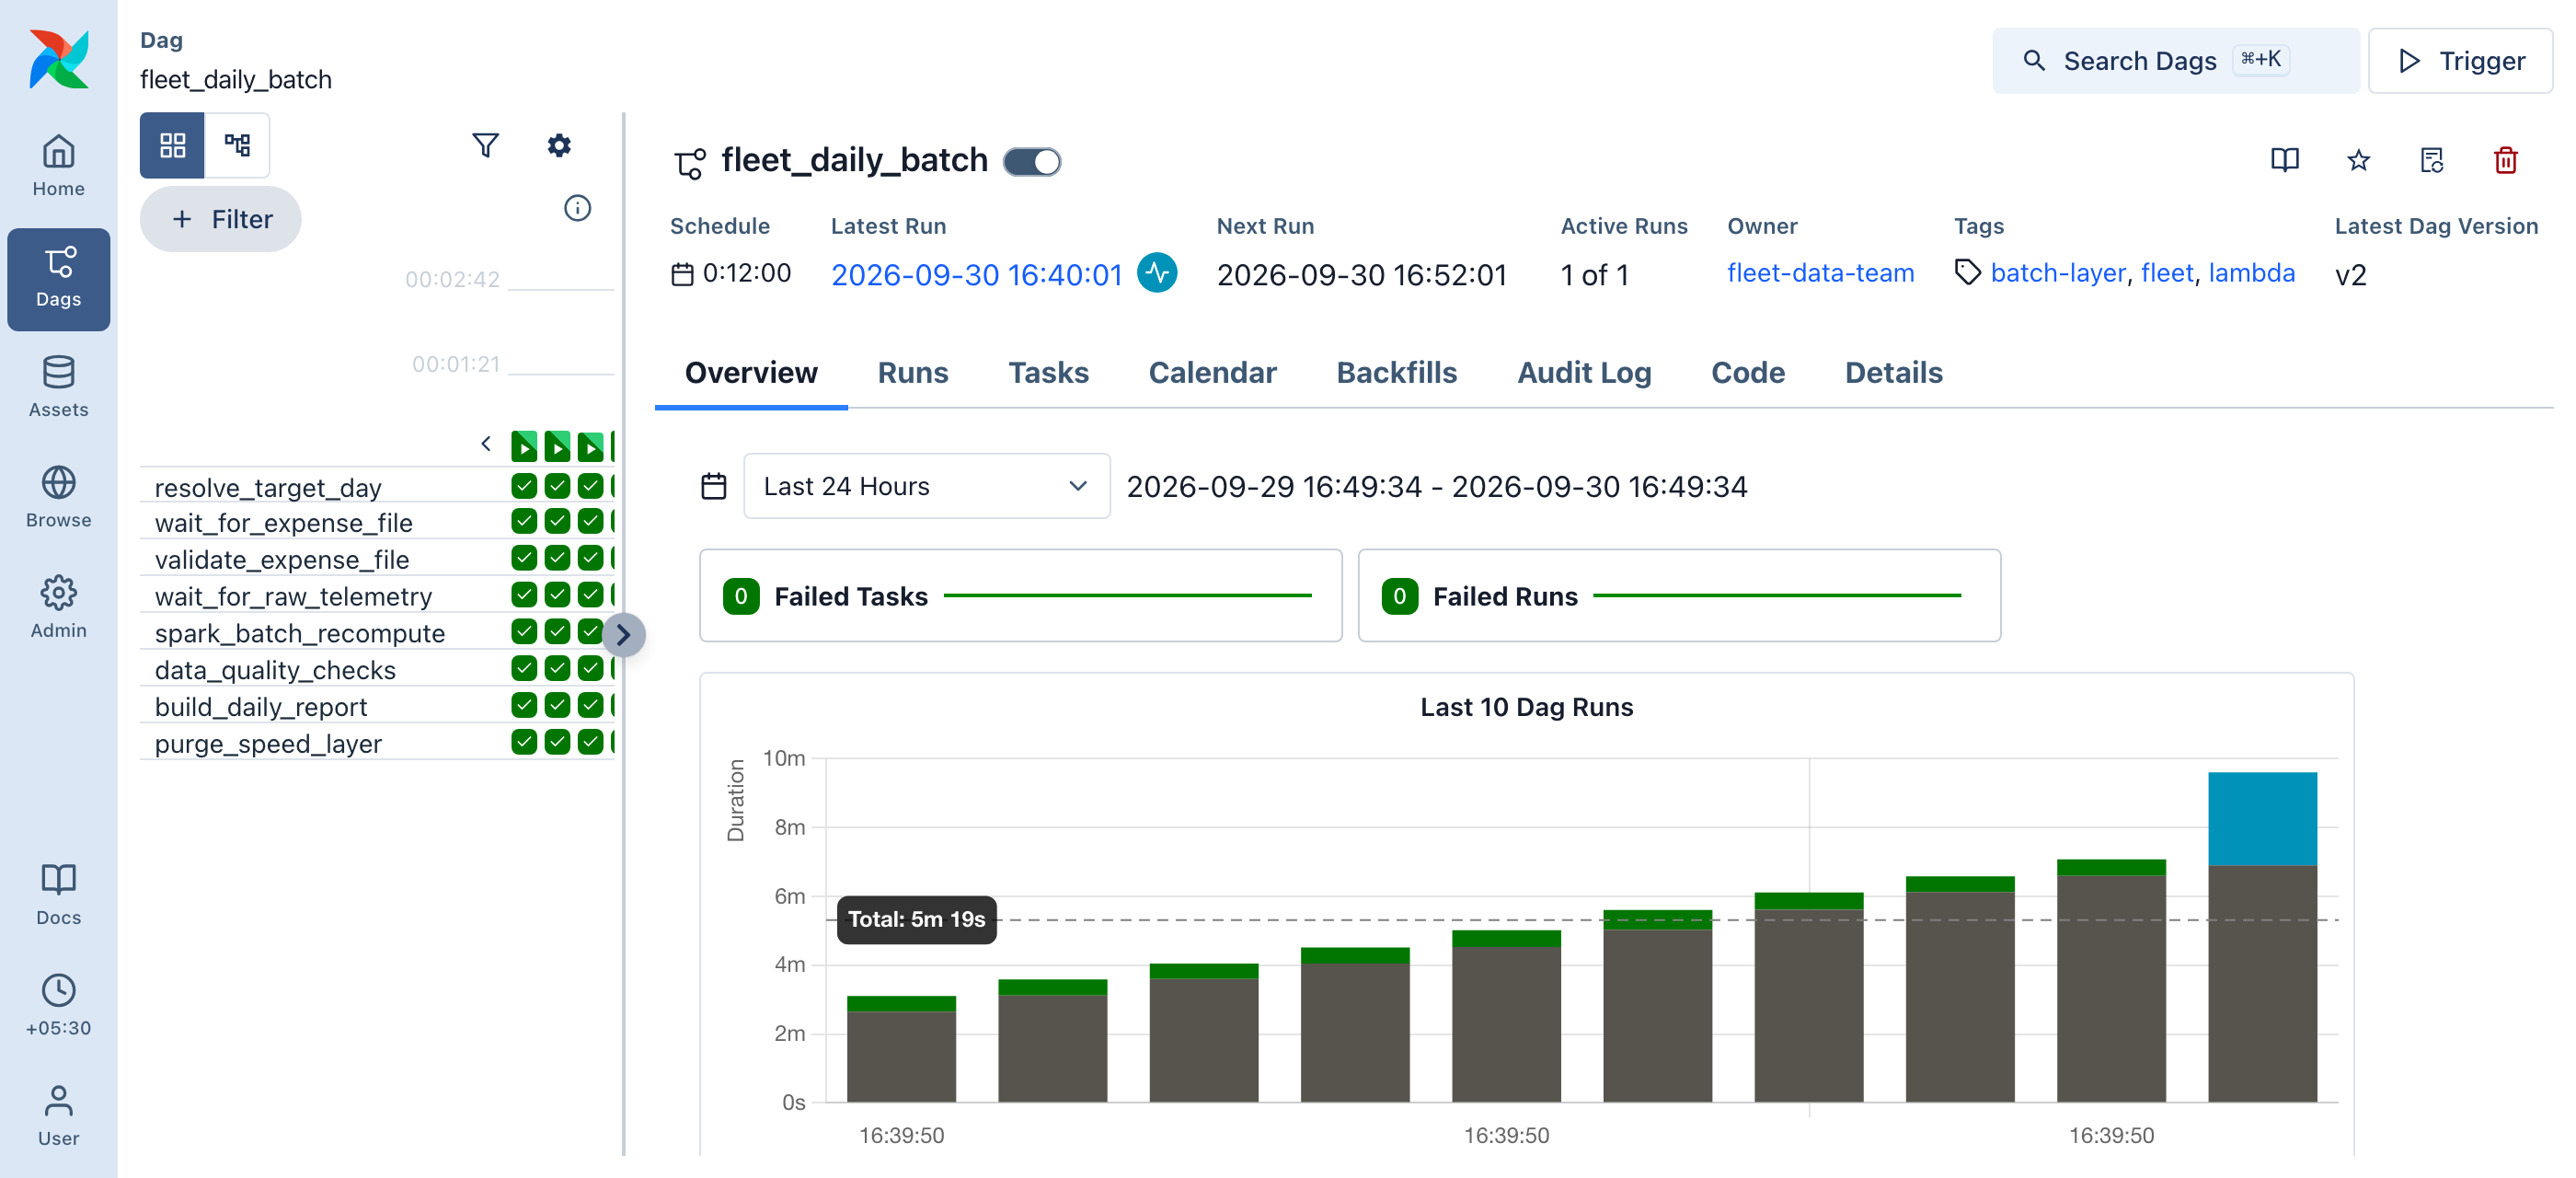
\includegraphics[width=0.85\textwidth]{figures/airflow_grid.png}
\caption{Airflow view of the DAG \code{fleet\_daily\_batch}. Each row is a task and each column is one run,
that is one simulated day. Green means success.}
\label{fig:dag}
\end{figure}

The Spark batch job reads only the master dataset. It removes invalid and repeated events over the whole
day, counts late events, and uses window functions on each vehicle's pings in time order to measure minutes
on a trip, minutes idle and the longest idle streak. It checks every cost row (numbers, dates, known
vehicles, repeated records). Bad rows go to a quarantine table with a reason. Then it joins the day's
telemetry with the costs. The profit of a vehicle for one day is:
\[
\text{net profit} = \text{fares} - 0.30 \times \text{fares} - \text{fuel cost} - \text{maintenance cost}
\]
A vehicle is \emph{unprofitable} when its net profit is below zero and \emph{at risk} when its margin is below
15\%. It is \emph{becoming unprofitable} when it is unprofitable or at risk and its profit fell on two days
in a row, or when it was profitable yesterday and loses money today. Days with a garage service bill are
never counted, because one large bill is not a trend. The job also
writes plain-English reasons, such as ``high fuel cost'' or ``reported km differ from GPS by 32\%''. All
views of the day are replaced in one PostgreSQL transaction, so users never see half a day.

\subsection{Serving layer}
\label{sec:serving}
The serving layer has three parts. The \textbf{FastAPI service} offers the endpoints in
Table~\ref{tab:api} and a \code{/docs} page. \textbf{Grafana} has three provisioned dashboards: live fleet
operations, daily profitability and pipeline health. The \textbf{daily report} is an HTML page (with a CSV
file) for fleet managers.

\begin{table}[!htb]
\centering\small
\caption{Main API endpoints.}
\label{tab:api}
\begin{tabularx}{\textwidth}{@{}P{5.9cm} L@{}}
\toprule
\textbf{Endpoint} & \textbf{Answer} \\
\midrule
\code{/api/v1/fleet/realtime} & live fleet status, trips and fares today, fares by zone \\
\code{/api/v1/zones/hourly?date=} & zone by hour metrics (batch view for finished days, speed view for today) \\
\code{/api/v1/profitability/live} & profit projected for today from live fares and batch cost rates \\
\code{/api/v1/profitability/daily?date=} & exact profit of every vehicle for a finished day \\
\code{/api/v1/alerts} & idle alerts and pipeline alert notifications \\
\code{/api/v1/pipeline/status} & freshness of each layer, recent runs and dead letters \\
\code{/reports/\{date\}.html} & the daily report \\
\bottomrule
\end{tabularx}
\end{table}

The most important Lambda merge is the \textbf{live profit projection}. The speed layer knows today's fares
and kilometres, and the batch layer knows each vehicle's recent fuel cost per kilometre and maintenance per
day. The view \code{serving.v\_vehicle\_profit\_live} combines them to show which vehicles are losing money
\emph{today}, before today's cost file exists. This answers the second part of the business question during
the day, and the batch layer confirms it with exact numbers after midnight.

\section{Observability design}
A pipeline that only works is not enough. We must see when it stops working, and why. Our design follows
three questions: \emph{is data flowing?}, \emph{is it correct?} and \emph{is it on time?} Every stage answers
them with logs, metrics and alerts.

\subsection{Structured logging}
Every Python component (simulators, both Spark jobs, Airflow tasks and the API) writes one JSON object per
line to standard output with the same core keys: \code{ts}, \code{level}, \code{service}, \code{stage}
(ingestion, processing, storage, serving or orchestration) and \code{event}. Extra keys give context, such as
the micro-batch id, the Airflow run id or the simulated date. Spark's own Java logs use Spark's JSON layout,
and the Kafka client logs pass through the same JSON formatter. Because all stages use the same keys, one
\code{jq} filter can follow a problem through the whole pipeline. This is a real line from the speed layer:

\noindent\begin{minipage}{\linewidth}
\begin{Verbatim}[fontsize=\scriptsize,frame=single,framesep=2mm,rulecolor=\color{black!30}]
{"ts": "2026-09-30T08:39:41.660+00:00", "level": "INFO", "service": "spark-speed-layer",
 "stage": "processing", "event": "vehicle_state_batch", "batch_id": 173, "rows": 100,
 "valid": 99, "dead_letters": 1, "vehicles_updated": 20, "idle_alerts_opened": 0,
 "idle_alerts_resolved": 0, "stream_time": "2026-09-02 18:11:36", "e2e_latency_s": 2.05,
 "duration_ms": 1398}
\end{Verbatim}
\end{minipage}

\subsection{Metrics}
Prometheus scrapes every stage every 10 seconds. Table~\ref{tab:metrics} lists the most useful metrics.

\begin{table}[!htb]
\centering\small
\caption{Main metrics, grouped by pipeline stage.}
\label{tab:metrics}
\begin{tabularx}{\textwidth}{@{}P{2.2cm} P{5.4cm} L@{}}
\toprule
\textbf{Stage} & \textbf{Metric} & \textbf{Why we measure it} \\
\midrule
Ingestion & events sent per partition, send errors, delivery latency, time of the last cost file & Is data reaching Kafka? Did the partner file arrive? \\
Processing & input rows per second, micro-batch duration, state rows (from a Spark query listener) & Is Spark keeping up with its trigger? \\
Processing & offsets behind the latest offset (lag), rows dropped by the watermark & Is the speed layer falling behind or losing late data? \\
Storage & end-to-end latency from Kafka to PostgreSQL, rows written, replayed batches & Are the tables fresh, and are writes exactly once? \\
Orchestration & Airflow task results and scheduler heartbeat (StatsD), batch days behind & Is the batch layer running every day? \\
Serving & API request rate and latency, vehicles by status, idle minutes, loss-making vehicles & Is serving healthy, and what is the business state? \\
\bottomrule
\end{tabularx}
\end{table}

\subsection{Tracing and lineage}
Full distributed tracing (for example with Jaeger) needs more memory than our laptop has, so we built
light-weight tracing and lineage from ids that already exist. Every event has an \code{event\_id}, which is
also sent as the Kafka header \code{trace\_id}. The master dataset stores the Kafka topic, partition, offset
and append time of every event, so any number in a report can be traced back to the exact Kafka records.
\code{ops.speed\_batches} records every committed micro-batch, \code{ops.batch\_files} every partner file
with its checksum, and \code{ops.pipeline\_runs} every Airflow step with its inputs, outputs and timing.
Each batch view row also carries the Airflow run id that produced it.

\subsection{Alerts and health checks}
\label{sec:alerts}
Prometheus evaluates 14 rules. Alertmanager groups the alerts and sends them to a webhook in our API, which
writes them as JSON logs and stores them in \code{ops.alert\_notifications}. Airflow task failures are
stored in the same table by a failure callback, so there is one place to see all problems.
Table~\ref{tab:alerts} shows the main rules. Some alerts are hidden when their cause is already known. For
example, if the Spark container is down, the alert ``speed layer stale'' is not sent again.

\begin{table}[!htb]
\centering\small
\caption{Main alert rules (real seconds, simulated time in brackets).}
\label{tab:alerts}
\begin{tabularx}{\textwidth}{@{}P{4.7cm} L P{1.5cm}@{}}
\toprule
\textbf{Alert} & \textbf{Condition} & \textbf{Severity} \\
\midrule
NoTelemetryIngested & no event reached Kafka for 1 minute (2 hours) & critical \\
SpeedLayerStale & the speed layer wrote nothing for more than 60 s & critical \\
StreamingQueryDown, ServiceDown & a Spark query stopped, or a service does not answer & critical \\
KafkaConsumerLagHigh & a query is more than 2000 offsets behind & warning \\
EndToEndLatencyHigh & Kafka to PostgreSQL takes more than 20 s & warning \\
InvalidEventRateHigh & more than 5\% of events are invalid & warning \\
BatchLayerBehind & more than one finished day is not processed & critical \\
ExpenseFeedMissing & no partner file for 1.5 simulated days & critical \\
VehicleIdleTooLong & a vehicle is idle for more than 90 simulated minutes & warning \\
VehiclesBecomingUnprofitable & yesterday's report found vehicles that are becoming unprofitable & info \\
\bottomrule
\end{tabularx}
\end{table}

\textbf{Failure drill.} To test detection, we stopped the stream simulator for 215 real seconds (about
seven simulated hours) and timed each alert.
\DrillText{}

\section{Results}
We ran the full system for \NumDays{} simulated days (about \RunMinutes{} real minutes) on a MacBook with an
Apple M-series chip and 8\,GB of memory. This section shows what the system produced.

\subsection{Live operations (speed layer)}
Figure~\ref{fig:live} shows the top of the live Grafana dashboard. \LiveText{} The map shows each vehicle
by status (green on a trip, blue going to a pickup, orange idle). The charts show fares by pickup zone, trips
per simulated hour and the status of vehicles in each zone. Further down, the dashboard has a utilisation
heatmap by zone and hour, the open idle alerts and the profit projection for today, which is the Lambda
merge of Section~\ref{sec:serving}.

\begin{figure}[!htb]
\centering
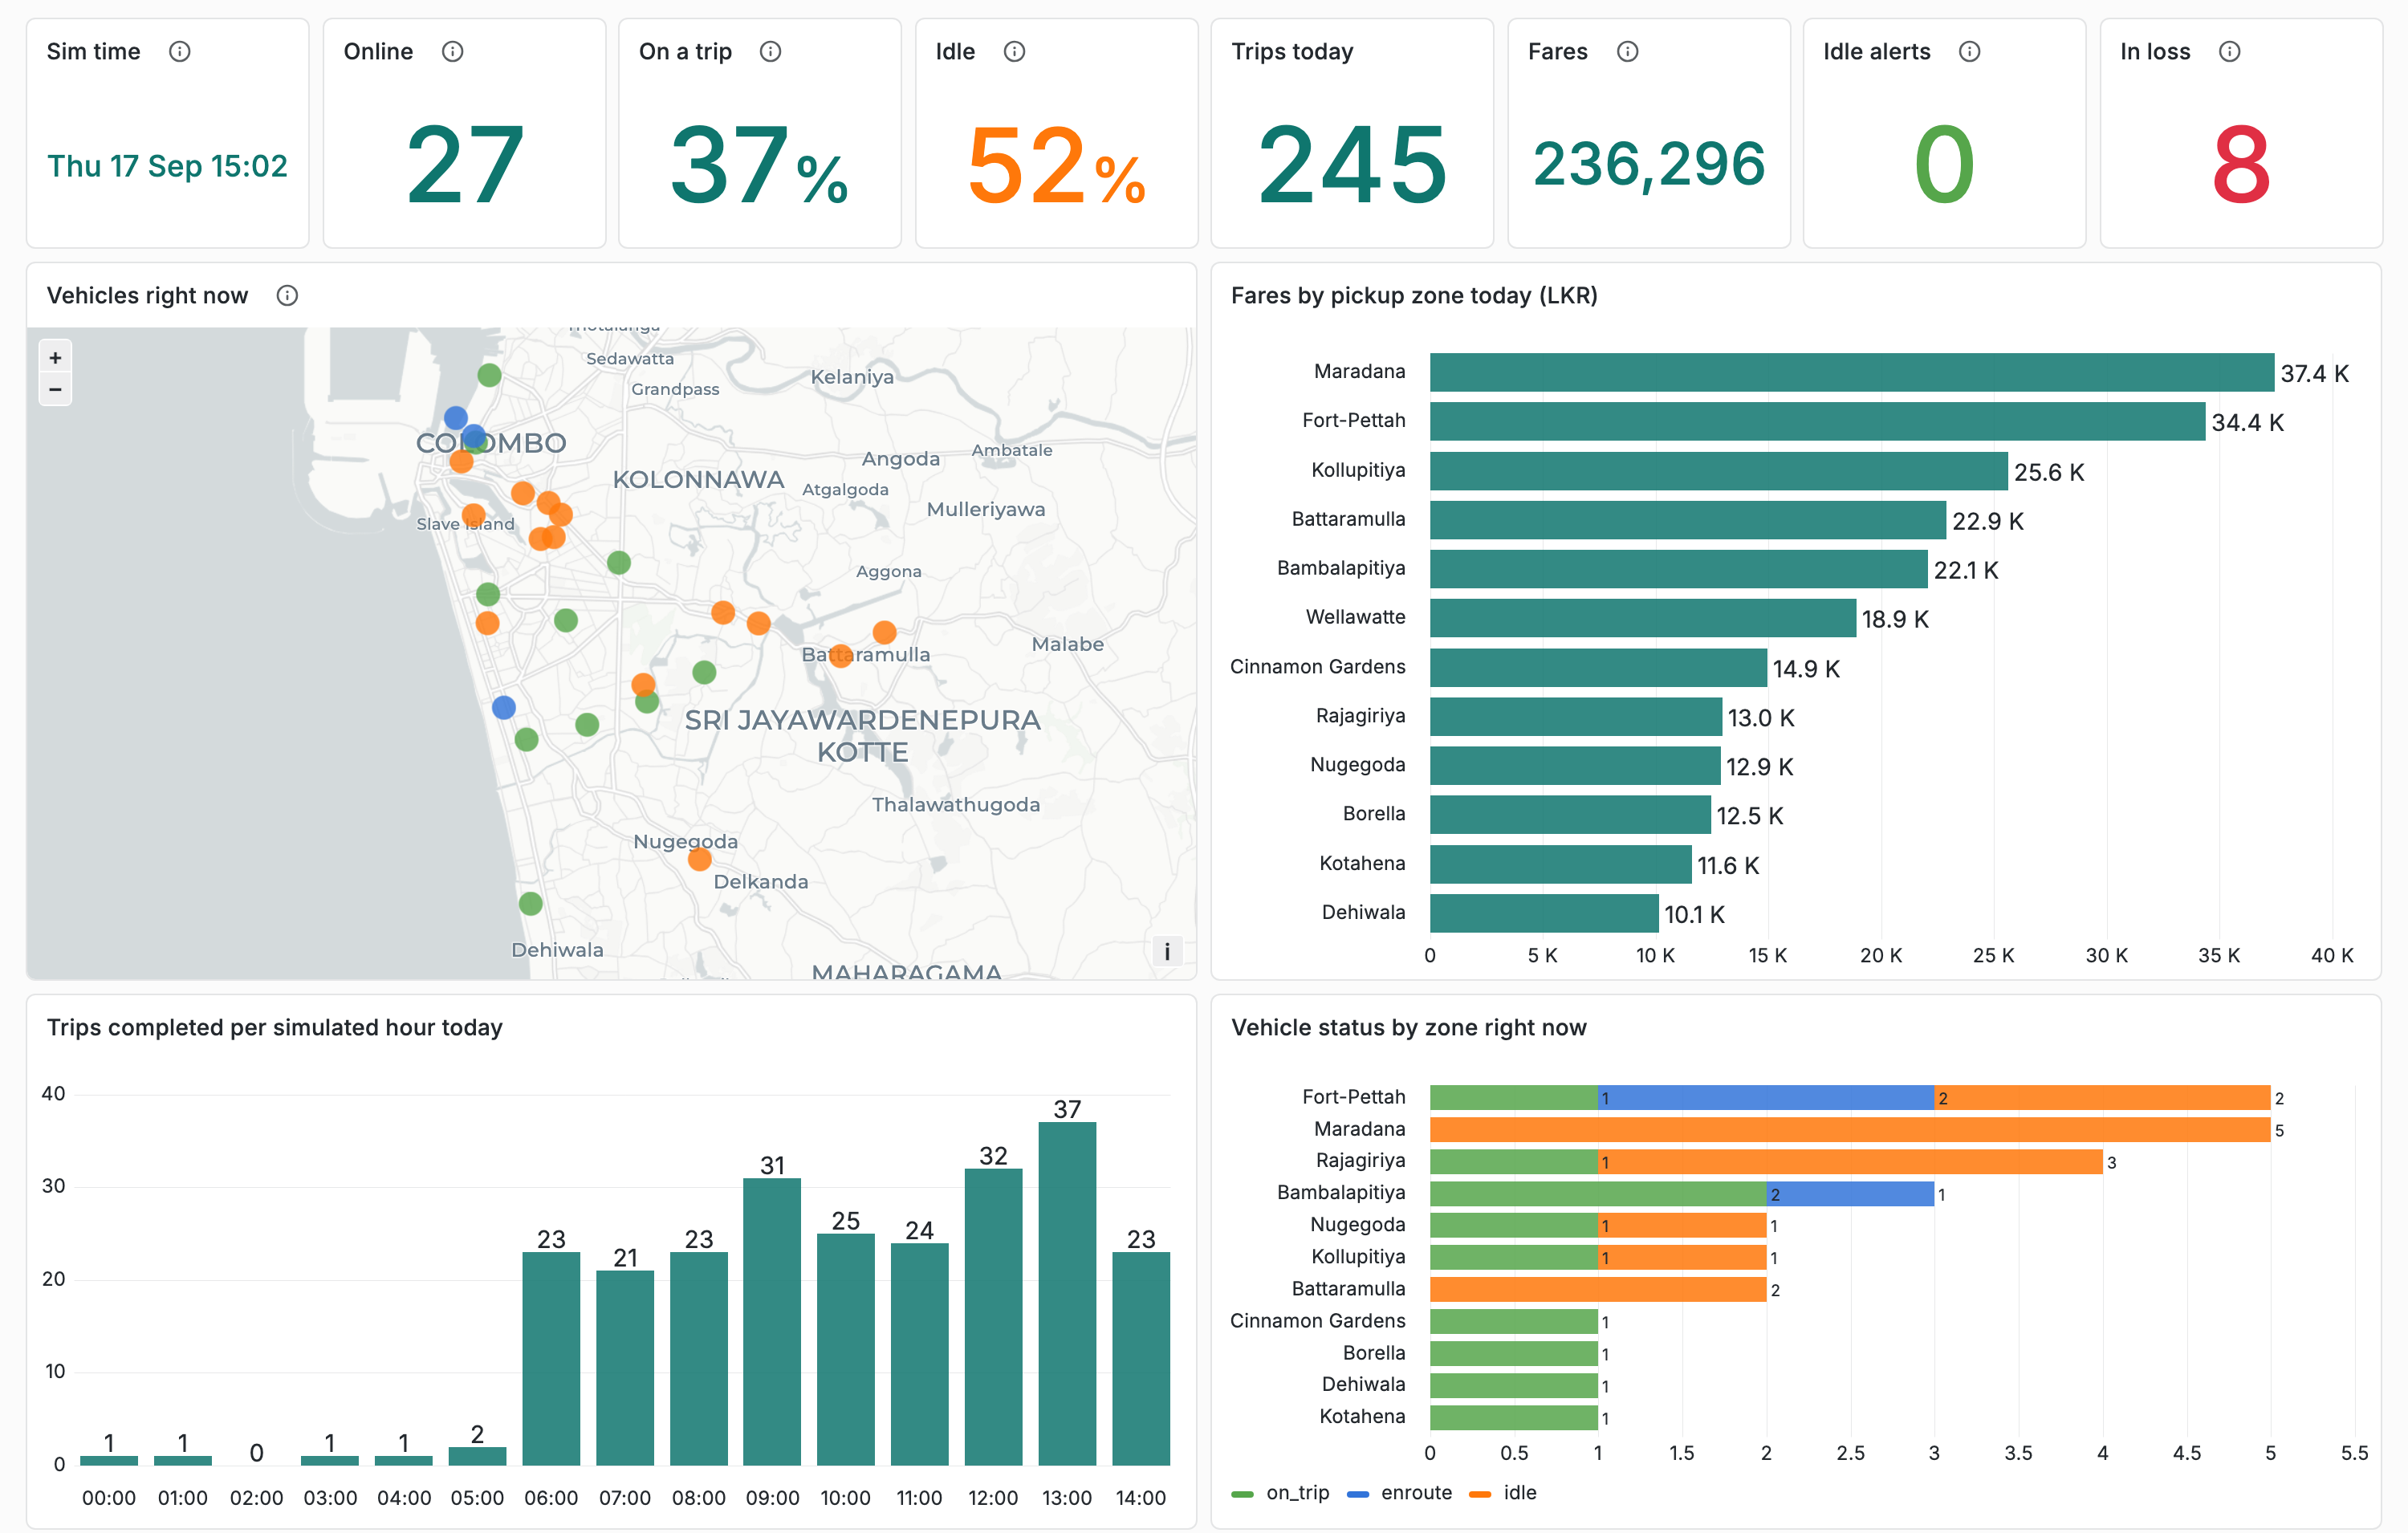
\includegraphics[width=0.92\textwidth]{figures/grafana_live.png}
\caption{Grafana dashboard ``Fleet operations (live)'', fed by the speed layer. It answers the first part of
the business question: utilisation and earnings by area and time of day, right now.}
\label{fig:live}
\end{figure}

\subsection{Daily profitability (batch layer)}
\label{sec:daily}
Table~\ref{tab:daily} gives the exact batch results for each day. Figure~\ref{fig:report} shows the top of
a daily report, and Figure~\ref{fig:trend} shows the daily net profit of the three problem vehicles compared
with the fleet average.

\begin{table}[!htb]
\centering\small
\caption{Exact daily results from the batch layer (money in LKR). Day 1 is 18 hours long.}
\label{tab:daily}
\begin{tabular}{@{}lrrrrrrrr@{}}
\toprule
\textbf{Day} & \textbf{Trips} & \textbf{Fares} & \textbf{Fuel + maint.} & \textbf{Net profit} & \textbf{Util. \%} & \textbf{Unprof.} & \textbf{At risk} & \textbf{Becoming} \\
\midrule
1 Sep & 489 & 483,550 & 154,962 & 183,523 & 41.6 & 0 & 2 & 0 \\
2 Sep & 506 & 497,098 & 155,046 & 192,923 & 42.2 & 1 & 0 & 0 \\
3 Sep & 461 & 451,097 & 159,128 & 156,640 & 39.4 & 2 & 0 & 1 \\
4 Sep & 467 & 455,089 & 187,856 & 130,707 & 39.0 & 4 & 1 & 0 \\
5 Sep & 434 & 438,988 & 155,254 & 152,037 & 38.3 & 4 & 0 & 1 \\
6 Sep & 459 & 464,670 & 193,060 & 132,209 & 40.4 & 3 & 1 & 0 \\
7 Sep & 451 & 443,800 & 167,604 & 143,056 & 39.4 & 3 & 0 & 0 \\
8 Sep & 472 & 453,180 & 181,166 & 136,060 & 38.7 & 3 & 1 & 1 \\
9 Sep & 447 & 443,783 & 197,836 & 112,812 & 38.6 & 6 & 1 & 0 \\
10 Sep & 466 & 462,885 & 152,639 & 171,381 & 39.5 & 2 & 0 & 0 \\
11 Sep & 457 & 456,118 & 154,960 & 164,323 & 40.0 & 2 & 0 & 1 \\
12 Sep & 469 & 469,820 & 170,924 & 157,950 & 40.7 & 3 & 0 & 1 \\
13 Sep & 467 & 457,249 & 175,066 & 145,009 & 39.0 & 2 & 1 & 1 \\
14 Sep & 454 & 442,848 & 159,057 & 150,937 & 38.0 & 3 & 0 & 2 \\
15 Sep & 470 & 462,878 & 194,604 & 129,411 & 39.5 & 5 & 0 & 1 \\
\bottomrule
\end{tabular}
\end{table}


\BusinessText{}

\begin{figure}[!htb]
\centering
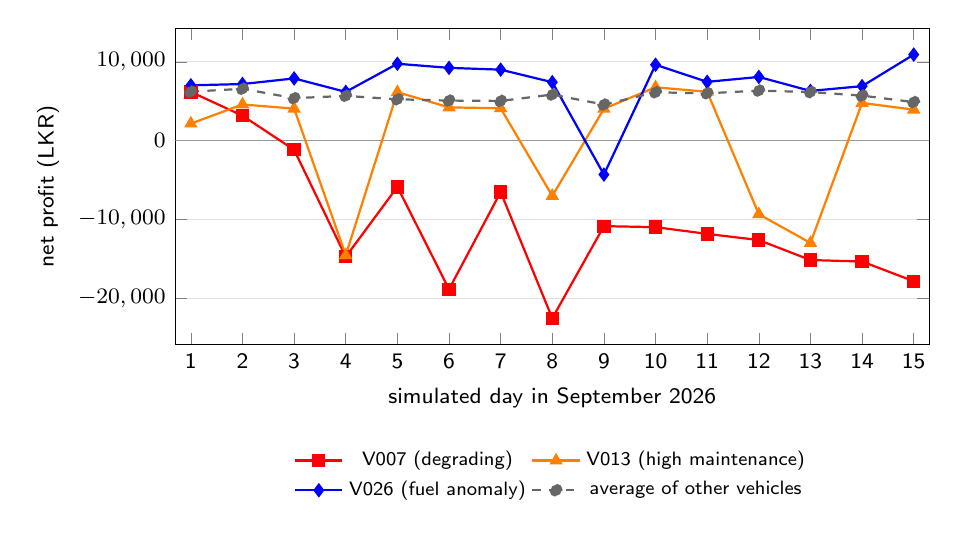
\begin{tikzpicture}
\begin{axis}[width=0.92\textwidth, height=5.6cm, font=\sffamily\footnotesize,
  xtick={1,2,3,4,5,6,7,8,9,10,11,12,13,14,15}, xticklabels={1,2,3,4,5,6,7,8,9,10,11,12,13,14,15}, xmin=0.7, xmax=15.3,
  xlabel={simulated day in September 2026}, ylabel={net profit (LKR)}, ymajorgrids, grid style={black!12},
  yticklabel style={/pgf/number format/fixed, /pgf/number format/1000 sep={,}},
  scaled y ticks=false, legend style={font=\sffamily\scriptsize, at={(0.5,-0.3)}, anchor=north,
  legend columns=2, draw=none}]
\addplot[black!40, thin, forget plot] coordinates {(0.7,0) (15.3,0)};
\addplot[red, mark=square*, thick] coordinates {(1,6199) (2,3182) (3,-1157) (4,-14735) (5,-5858) (6,-18855) (7,-6512) (8,-22536) (9,-10842) (10,-10968) (11,-11826) (12,-12607) (13,-15145) (14,-15331) (15,-17830)};
\addlegendentry{V007 (degrading)}
\addplot[orange, mark=triangle*, thick] coordinates {(1,2176) (2,4601) (3,4073) (4,-14521) (5,6169) (6,4232) (7,4119) (8,-7005) (9,4059) (10,6783) (11,6212) (12,-9324) (13,-12975) (14,4795) (15,3947)};
\addlegendentry{V013 (high maintenance)}
\addplot[blue, mark=diamond*, thick] coordinates {(1,7033) (2,7196) (3,7909) (4,6201) (5,9771) (6,9249) (7,9023) (8,7427) (9,-4294) (10,9641) (11,7474) (12,8095) (13,6323) (14,6928) (15,10933)};
\addlegendentry{V026 (fuel anomaly)}
\addplot[black!60, dashed, thick, mark=*] coordinates {(1,6226) (2,6591) (3,5401) (4,5695) (5,5258) (6,5096) (7,5053) (8,5858) (9,4588) (10,6145) (11,6017) (12,6362) (13,6178) (14,5724) (15,4902)};
\addlegendentry{average of other vehicles}
\end{axis}
\end{tikzpicture}

\caption{Daily net profit of the vehicles with special profiles and the average of all other vehicles
(batch layer, LKR).}
\label{fig:trend}
\end{figure}

\begin{figure}[!htb]
\centering
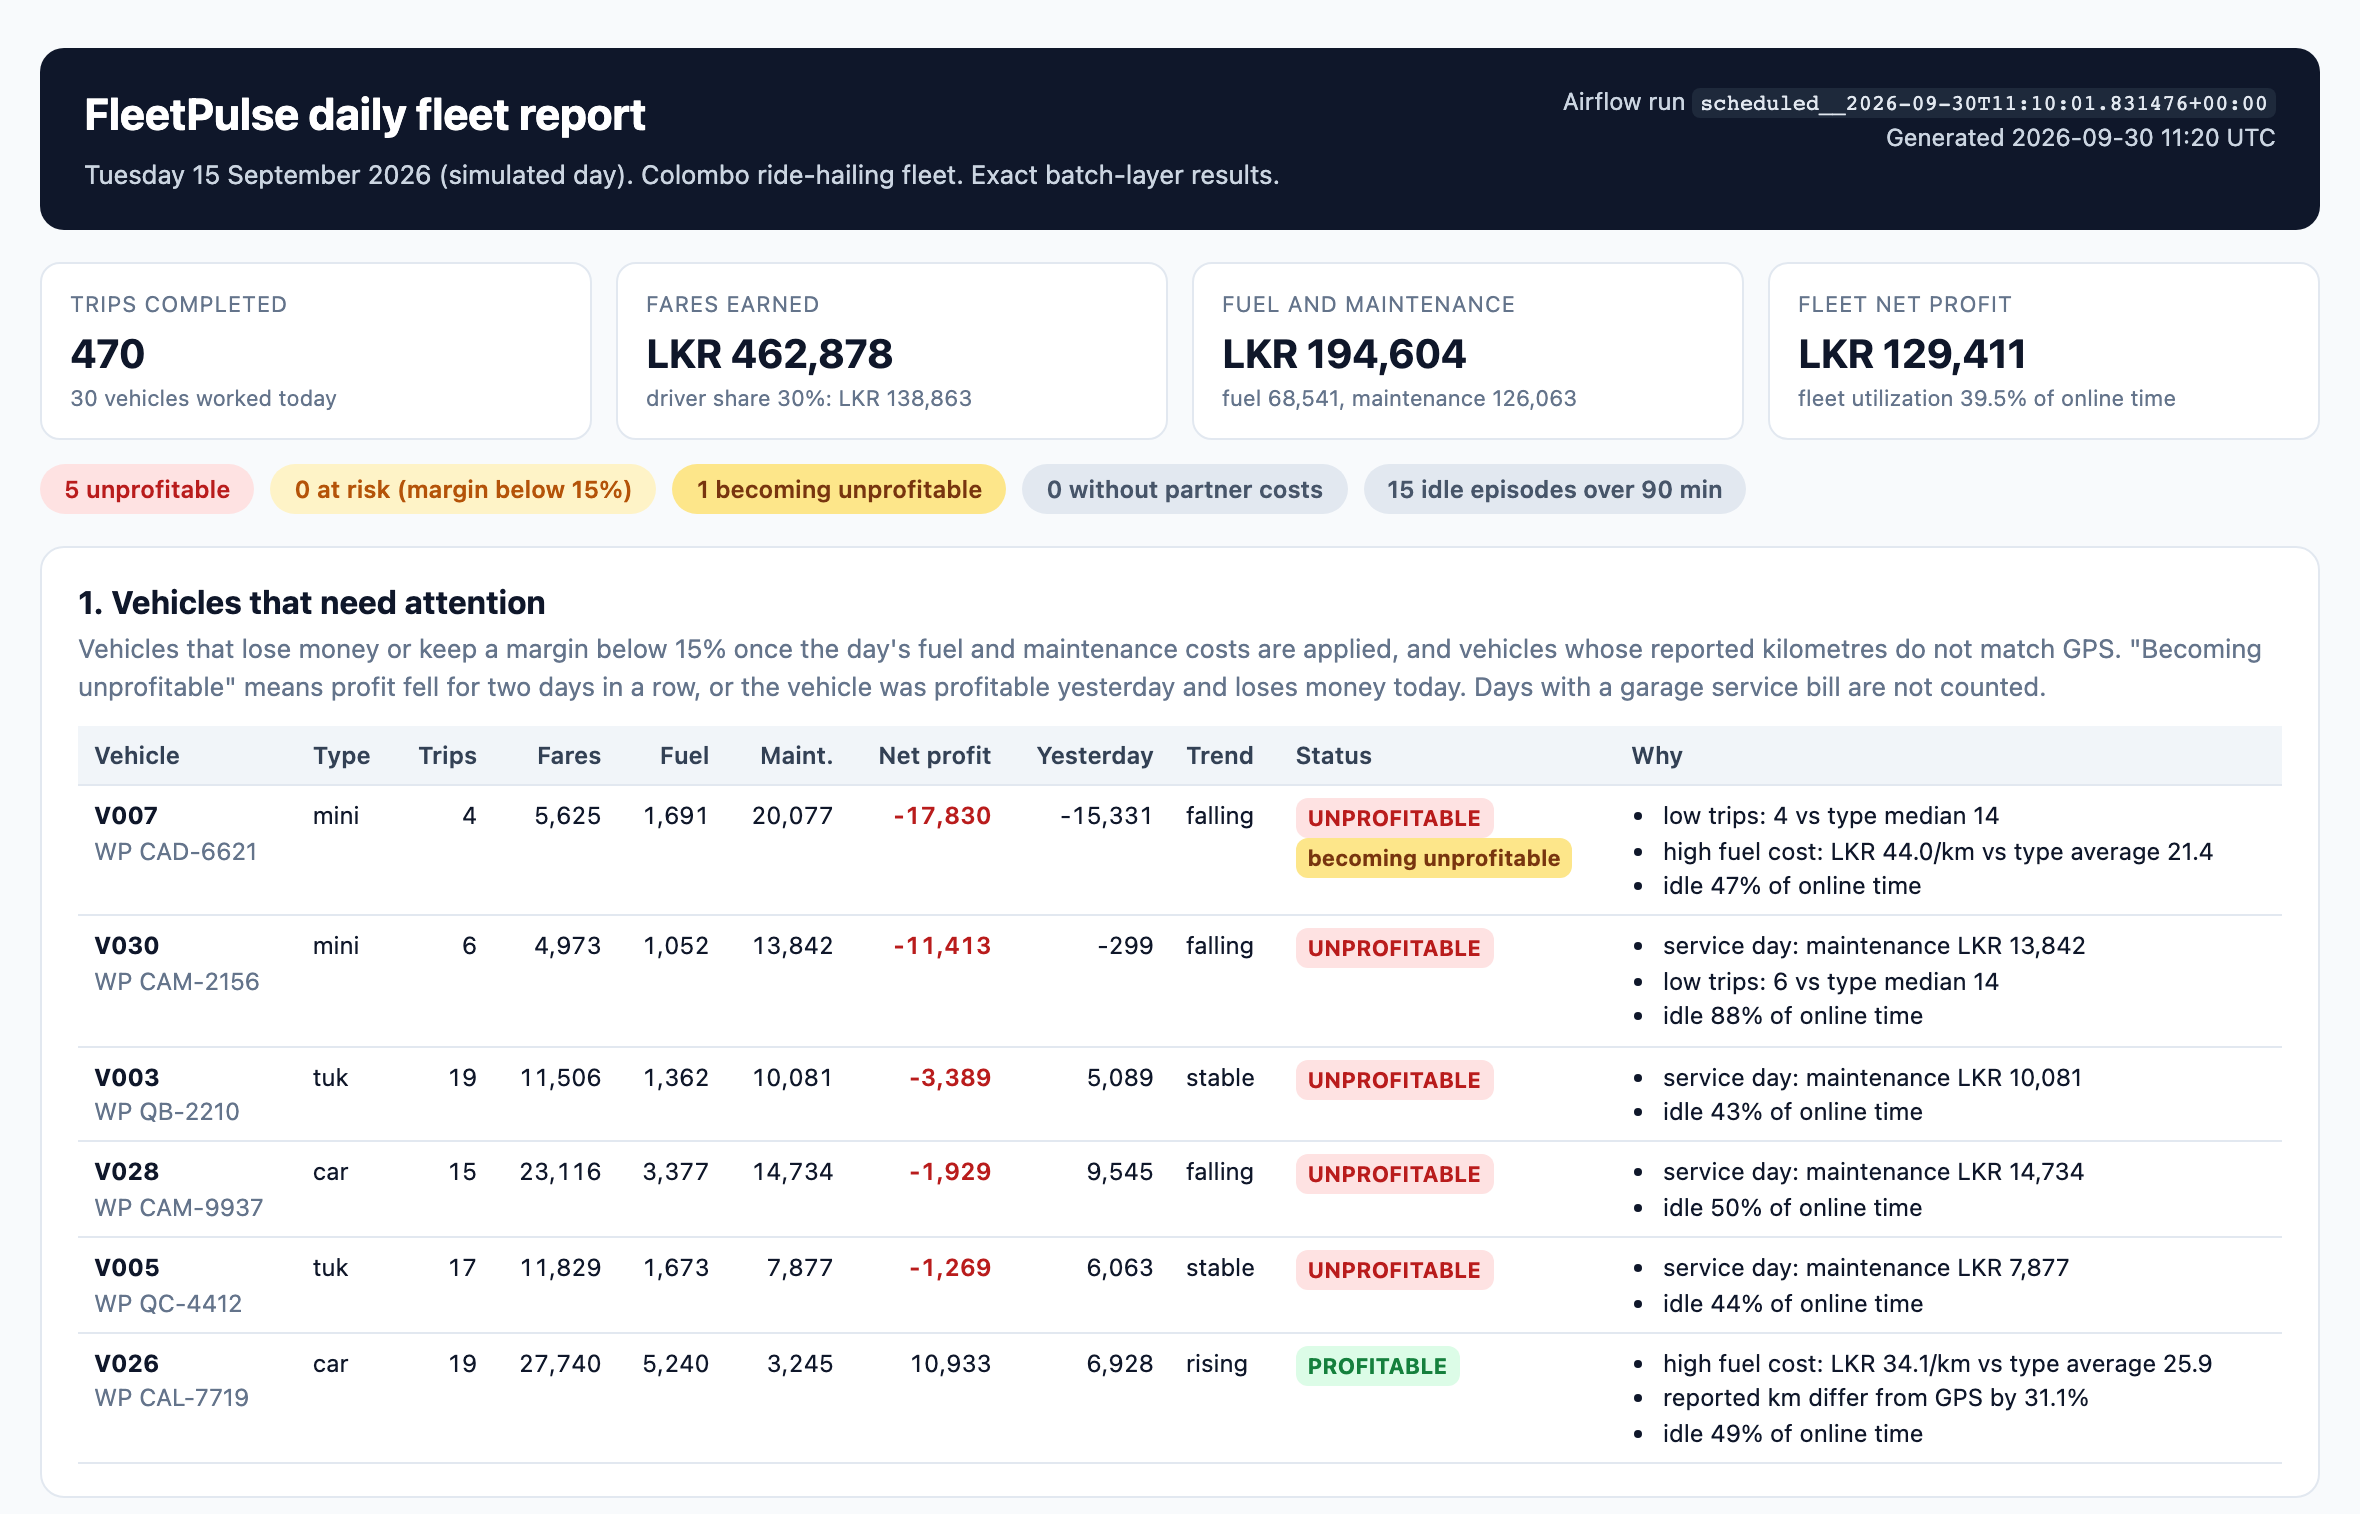
\includegraphics[width=0.86\textwidth]{figures/daily_report_top.png}
\caption{Top of the daily HTML report built by Airflow for day \ReportDay{}. It lists the vehicles that
need attention and explains why, which answers the second part of the business question.}
\label{fig:report}
\end{figure}

\subsection{Speed layer compared with the batch layer}
\label{sec:reconciliation}
After each batch run the DAG compares the day's totals from both layers (Table~\ref{tab:recon}). The speed
layer missed some events because they arrived after its 10-minute watermark. The batch layer read the
complete day, so it recovered them. \ReconText{}

\begin{table}[!htb]
\centering\small
\caption{Speed layer compared with the batch layer, and what the batch layer cleaned, per day (days 2 to 15, lowest, average and highest day).}
\label{tab:recon}
\begin{tabularx}{\textwidth}{@{}L rrr@{}}
\toprule
\textbf{Measure per day} & \textbf{Lowest} & \textbf{Average} & \textbf{Highest} \\
\midrule
Trips missed by the speed layer & 0 & 1.9 & 5 \\
Fares missed by the speed layer (\% of batch fares) & 0.00 & 0.42 & 1.11 \\
Pings missed by the speed layer (\% of batch pings) & 0.08 & 0.31 & 0.66 \\
Late events (more than 10 simulated minutes) & 55 & 174 & 256 \\
Repeated events removed & 84 & 109 & 134 \\
Invalid events removed & 24 & 35 & 47 \\
Bad cost rows put in quarantine & 0 & 1.6 & 3 \\
\bottomrule
\end{tabularx}
\end{table}


\subsection{Orchestration and pipeline health}
Figure~\ref{fig:dag} in Section~\ref{sec:batch} shows the Airflow runs, and Figure~\ref{fig:health} shows the pipeline
health dashboard. \HealthText{}

\begin{figure}[!htb]
\centering
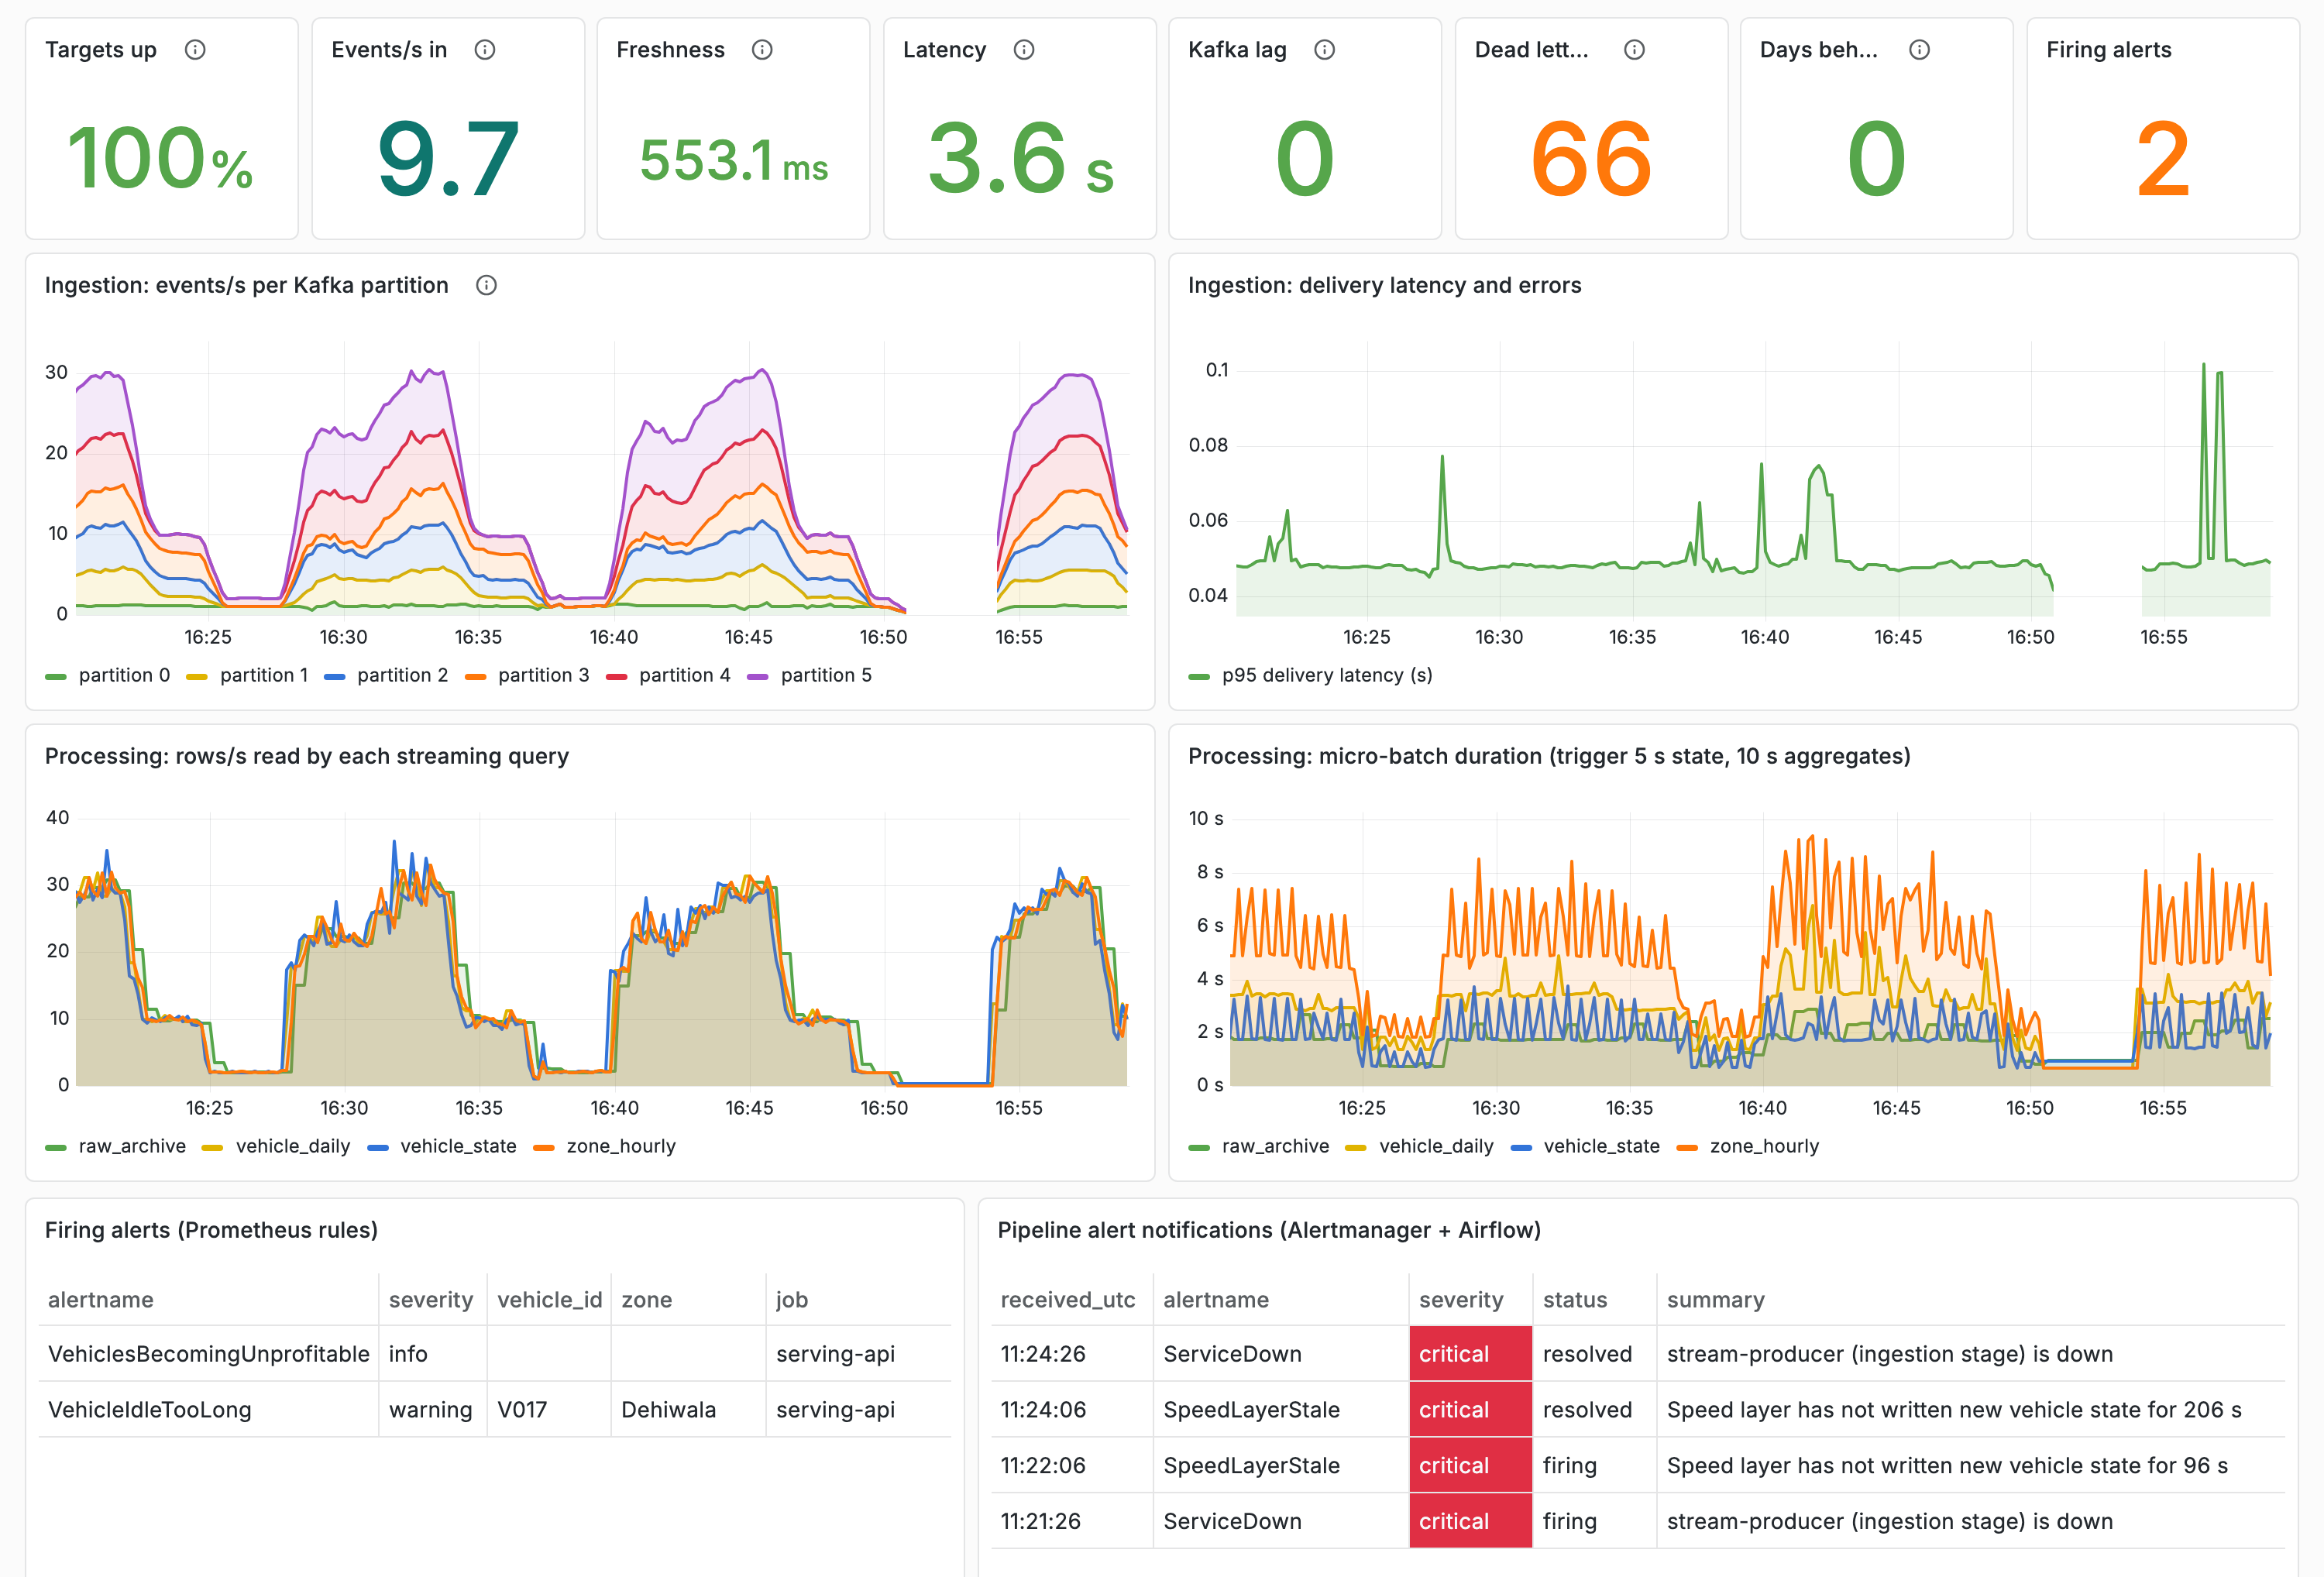
\includegraphics[width=0.92\textwidth]{figures/grafana_pipeline.png}
\caption{Grafana dashboard ``Pipeline health'' during the failure drill (top rows and alert tables). The gap
from 16:51 to 16:54 in the charts (Sri Lanka time) is the drill. The table on the right lists the alert
notifications that reached the API, with times in UTC. Lower rows (latency, lag, Airflow tasks and the run
audit trail) are not shown.}
\label{fig:health}
\end{figure}

\subsection{Performance on one laptop}
Table~\ref{tab:perf} shows speed and resource use measured during the run.

\begin{table}[!htb]
\centering\small
\caption{Speed and resource use during the run.}
\label{tab:perf}
\begin{tabularx}{\textwidth}{@{}L r@{}}
\toprule
\textbf{Measure} & \textbf{Value} \\
\midrule
Events per second into Kafka (average) & 15.8 \\
Producer delivery latency, 95th percentile & 48\,ms \\
End-to-end latency Kafka to PostgreSQL, vehicle state (average) & 2.3\,s \\
End-to-end latency, oldest record in a vehicle-state batch (maximum) & 8.2\,s \\
End-to-end latency, zone by hour windows (average) & 5.3\,s \\
Micro-batch duration: vehicle state and zone by hour (average) & 2.0\,s and 4.9\,s \\
Largest Kafka lag of any streaming query & 0 offsets \\
Spark batch job for one simulated day (average) & 20\,s \\
\midrule
\multicolumn{2}{@{}p{\dimexpr\textwidth\relax}@{}}{\raggedright\textbf{Batch job steps (average):} spark start 4\,s, validate expenses 1\,s, clean telemetry 8\,s, join and profitability 3\,s, write curated parquet 3\,s, publish postgres 1\,s} \\
\multicolumn{2}{@{}p{\dimexpr\textwidth\relax}@{}}{\raggedright\textbf{Memory per container:} airflow 438, alertmanager 43, api 41, batch-producer 10, grafana 232, kafka 77, postgres 64, prometheus 132, spark-streaming 786, statsd-exporter 36, stream-producer 37 (MiB, total 1.9\,GiB)} \\
\bottomrule
\end{tabularx}
\end{table}


\subsection{Testing}
The project has 39 automated tests (\code{pytest}), which run in their own Docker image. They cover the
simulated clock, the zone lookup, the fleet model, the cost file and its manifest, the idle-streak logic,
every validation rule, the zone metrics and profit rules in Spark, and a full batch-layer run on a small
synthetic day with known answers. One test checks that the Spark profit rules give the same answer as the
Python rules, which protects the two Lambda code paths from drifting apart. All 39 tests pass.

\section{Limitations, trade-offs and production changes}

\subsection{Limitations}
\begin{itemize}
\item \textbf{Single nodes.} Kafka has one broker with replication factor 1, and Spark runs in local mode. A
broker failure would stop ingestion, and one machine limits the throughput.
\item \textbf{Simple model.} Vehicles move in straight lines, and zones are nearest-centre areas on a coarse
grid, so a point near a zone border can fall in the wrong zone.
\item \textbf{Estimated lateness.} The batch layer counts an event as late when it arrived more than
10 simulated minutes after it happened. This is close to, but not exactly, what the speed layer dropped.
\item \textbf{Light tracing and local security.} We trace with ids and lineage tables instead of OpenTelemetry
and Jaeger. Passwords are in an \code{.env} file, and Kafka and PostgreSQL use no TLS.
\item \textbf{Limited memory.} The full stack needs most of the memory that Docker can use on an 8\,GB
laptop, so heavy desktop apps make the batch runs slower.
\end{itemize}

\subsection{Trade-offs we accepted}
\begin{itemize}
\item \textbf{Two code paths} give exact money numbers and cheap recomputing. Shared code and a parity test
reduce the risk that they drift apart.
\item \textbf{A 10-second trigger} for the aggregate queries instead of 5 seconds halves the CPU they use.
\item \textbf{A 10-minute watermark} keeps state small and dashboards fresh, but the speed layer drops some
late events. The batch layer counts them after midnight.
\item \textbf{Collecting to the driver.} The \code{vehicle\_state} query collects each small micro-batch
(about 100 rows) to the Spark driver. This is much faster than several Spark jobs per batch, and the input
cap of 5000 offsets per trigger keeps it safe.
\item \textbf{Kafka native image.} It saves memory, but Apache says it is for development and testing. The
Java image is a drop-in replacement.
\end{itemize}

\subsection{What we would change at production scale}
\begin{itemize}
\item \textbf{Kafka:} a cluster of at least three brokers with replication factor 3, and a schema registry
with Avro or Protobuf schemas for the events.
\item \textbf{Spark:} a cluster (Kubernetes or a managed service) with more partitions and the RocksDB state
store for large state.
\item \textbf{Master dataset:} S3 or HDFS with an open table format such as Delta Lake or Apache Iceberg,
and regular compaction of the small files that streaming creates.
\item \textbf{Airflow:} the Kubernetes or Celery executor, with Spark batch jobs started on the cluster.
\item \textbf{Zones:} a real geo index, for example H3 cells or zone polygons.
\item \textbf{Operations:} central logs (Loki or Elasticsearch), OpenTelemetry tracing, alerts by e-mail,
SMS or Slack, a secret manager and TLS everywhere.
\end{itemize}

\section{Conclusion}
FleetPulse shows that a Lambda architecture fits a ride-hailing fleet that has both a live GPS stream and a
daily cost file. The speed layer gives utilisation, fares and idle alerts within seconds. The batch layer
recomputes each day exactly, joins it with the partner costs and finds vehicles that are becoming
unprofitable, with clear reasons. Shared Spark code, a parity test and reconciliation between the layers keep
the two paths in step. Logs, metrics, alerts and lineage tables make every stage observable, and one Docker
Compose command starts the whole system on a laptop.

\section{Individual contributions}
All three members took part in the design discussions, the testing and the writing of this report. The main
responsibilities were shared as shown in Table~\ref{tab:contrib}.

\begin{table}[H]
\centering\small
\caption{Individual contributions.}
\label{tab:contrib}
\begin{tabularx}{\textwidth}{@{}p{5.2cm} L@{}}
\toprule
\textbf{Member} & \textbf{Main work} \\
\midrule
Arivanan V. (EG/2021/4414) & Data simulators (fleet model, streaming source and daily-batch source) and Kafka ingestion (topics, partitions, producer settings) \\
Shageethpratheep V. (EG/2021/4809) & Spark speed layer and batch layer, shared transformation module, Lambda architecture decision \\
Shayanthavi T. (EG/2021/4811) & Airflow orchestration, PostgreSQL design, FastAPI serving layer, Grafana dashboards and observability \\
All three members & Testing, demo, and this report \\
\bottomrule
\end{tabularx}
\end{table}

\begin{thebibliography}{9}
\small
\bibitem{marz2015} N. Marz and J. Warren, \emph{Big Data: Principles and Best Practices of Scalable Real-Time
Data Systems}. Manning Publications, 2015.
\bibitem{kreps2014} J. Kreps, ``Questioning the Lambda Architecture,'' O'Reilly Radar, July 2014.
\bibitem{kleppmann2017} M. Kleppmann, \emph{Designing Data-Intensive Applications}. O'Reilly Media, 2017.
\bibitem{spark} Apache Software Foundation, ``Structured Streaming Programming Guide,'' Apache Spark 4.1
documentation, 2026.
\bibitem{kafka} Apache Software Foundation, ``Apache Kafka Documentation,'' version 4.3, 2026.
\bibitem{airflow} Apache Software Foundation, ``Apache Airflow Documentation,'' version 3.3, 2026.
\end{thebibliography}


\end{document}
